%! TeX program = lualatex
%---------------------------ALLGEMEINE IMPORTS-------------------------------------
\documentclass[12pt,english,ngerman]{scrartcl}

\usepackage{iftex}

% text input and font
\ifluatex  % LuaLaTeX
    \usepackage{fontspec}
    % main font automatically: Latin Modern
    %\setmonofont{Consolas}
    % \newfontfamily{\Consolas}{Consolas}
\else  % pdfLaTeX
    \usepackage[utf8]{inputenc}  % input in UTF-8
    \usepackage[T1]{fontenc}  % output in T1 fonts (west European encoding)
    \usepackage{lmodern}  % Latin modern font for main text
    \usepackage[mono]{zi4}  % Consolas font for monospaced text
    % \newfontfamily{\Consolas}{\fontfamily{zi4}}
\fi

% text processing
\usepackage{babel}  % language package
\usepackage[intlimits]{mathtools}  % upgrade of amsmath (automatically loaded) - \int^_ like \limits^_
\usepackage{amssymb}  % upgrade of amsfonts (American Math Society)
\usepackage{amstext}  % \text command in math environments
%\usepackage{bm}  % bold math fonts
% \LetLtxMacro{\svqty}{\qty}
% \usepackage{physics}  % macros for easier typesetting of physical formulas
% \LetLtxMacro{\qty}{\svqty}
\usepackage{letltxmacro}  % \let command for robust macros (new sqrt)
\usepackage{chemformula}  % typeset chemical formulas
\usepackage{microtype}


% page geometry
\usepackage{scrlayer-scrpage}  % page formatting with KOMA options
\usepackage[paper=a4paper, hmargin=3cm, vmargin=2.5cm, includehead, includefoot, head=29pt]{geometry}  % horizontal: 3cm, vertical: 2.5cm strict with or without headers and footers
\usepackage{tabto}  % tab stops
\NumTabs{8}  % 8 equally spaced of \textwidth tab stops



% floats
\usepackage[hypcap=false, labelfont=bf]{caption, subcaption}  % caption editing - hypcap warning with hyperref
\usepackage{float}  % for [H] (forced here) specifier
\usepackage{tabularray}
\usepackage{diagbox}  % table cells with diagonal lines


% graphical input
\usepackage{graphicx}  % input JPEG, PNG, PDF, etc.
\usepackage{pdfpages}  % input PDF as whole pages
\usepackage{lastpage}  % reference to last page
\usepackage{pgfplots}  % for tikzplotlib
\usepgfplotslibrary{groupplots,dateplot}
\usetikzlibrary{patterns,shapes.arrows}
\pgfplotsset{compat=newest}
\usepackage{import}


% text
\usepackage[locale=DE, uncertainty-mode=separate]{siunitx}  % SI units, German formatting - \pm stays \pm instead of ..(.)
\let\svqty\qty %dont import physics before siunitx is loaded
\usepackage{physics}
\let\qty\svqty
\usepackage{icomma}  % no space after commas instead of English points) in decimal values
\usepackage{enumitem}  % better enumerating with style options
\usepackage{nicefrac}  % inline-fractions in n/d-style
\usepackage{xcolor}  % custom colors
\usepackage{listings, scrhack}  % code display; listings in combination with KOMA
\usepackage{fancyvrb}  % Verbatim environment with better options (capital V!)

\usepackage{listings}

% literacy
\usepackage[bibencoding=auto,backend=biber,autolang=other]{biblatex}  % backend=Biber is standard
\usepackage{csquotes}  % better quotation - should also be used in combination with package babel (warning)
\usepackage{xurl}  % breaks links - after BibLaTeX, but before hyperref!
\usepackage[hidelinks]{hyperref}  % produces most errors, last to load
\usepackage{bookmark}


% KOMA setups
% header and footer
\pagestyle{scrheadings}  % KOMA style
\clearpairofpagestyles  % reset
\setkomafont{pageheadfoot}{\normalfont}  % standard font in header and footer
\setlength{\headheight}{29pt}  % just look at the warning
\cfoot{\pagemark{} / \pageref*{LastPage}}  % center foot - *: ref but no hyperlink
% {}: empty statement
% \ : protected space
% \,: small space
\DeclareTOCStyleEntry{dottedtocline}{section}  % sections in TableOfContents with dotted lines
\KOMAoptions{parskip=half-}  % paragraphs with half a line height space instead of indentation, last line with no special treatment


% package setups

% biblatex
%\addbibresource{files/JabRef_Database/physics.bib}
% \addbibresource{transistor.bib}

% rewrite names (babel overwrites German with standard English names, therefore at document beginn [after everything is loaded])
\AtBeginDocument{\renewcommand{\refname}{Literaturverzeichnis}}
% others:
% \contentsname
% \listtablename
% \listfigurename


% xcolor
\definecolor{code_keyword}{HTML}{A06E9D}
\definecolor{code_string}{HTML}{AD6E3E}
\definecolor{code_comment}{HTML}{6A9955}
%\definecolor{code_basic}{HTML}{D4D4D4}
%\definecolor{code_background}{HTML}{1E1E1E}

% siunitx
\DeclareSIUnit{\dig}{dig}  % digits for uncertainty of electronical measurement devices
\sisetup{locale = DE}  % deutschsprachige SI-Konvention
\sisetup{per-mode = fraction}
\DeclareSIUnit{\px}{px}
\DeclareSIUnit{\strich}{|||}

%Eigene Commands
\newcommand{\der}[2]{\frac{\mathrm{d}#1}{\mathrm{d}#2}}
\newcommand{\pder}[2]{\frac{\partial #1}{\partial #2}}

% listings
\lstdefinestyle{python}{
    %basicstyle=\Consolas\footnotesize,%\color{code_basic},  % \footnotesize contains \selectfont implicitly
    %backgroundcolor=\color{code_background},
    commentstyle=\color{code_comment},
    keywordstyle=\bfseries\color{code_keyword},
    numberstyle=\tiny,
    stringstyle=\color{code_string},
    breakatwhitespace=false,
    breaklines=true,
    captionpos=b,
    keepspaces=true,
    numbers=left,
    numbersep=5pt,
    showspaces=false,
    showstringspaces=false,
    showtabs=false,
    tabsize=2,
}
\lstset{style=python}
\ifPDFTeX
    \renewcommand*{\ttdefault}{lmvtt}  % Latin Modern Typewriter Proportional
\fi


% new sqrt
% https://en.wikibooks.org/wiki/LaTeX/Mathematics
\makeatletter
\let\oldr@@t\r@@t
\def\r@@t#1#2{%
    \setbox0=\hbox{$\oldr@@t#1{#2\,}$}\dimen0=\ht0
    \advance\dimen0-0.2\ht0
    \setbox2=\hbox{\vrule height\ht0 depth -\dimen0}%
    {\box0\lower0.4pt\box2}}
\LetLtxMacro{\oldsqrt}{\sqrt}
\renewcommand*{\sqrt}[2][\ ]{\oldsqrt[#1]{#2} }
\makeatother


% own commands
% \newcommand* can't contain multiple lines
% \newcommand can
\newcommand*{\mup}[1]{\ensuremath{\text{\textup{#1}}}}  % upright normal font in math mode
\newcommand*{\inkgraphics}[3][\linewidth]{\def\svgwidth{#1}\import{#2}{#3}}


% tabularray
% imports_and_setups{
%     expl3,
%     xparse,
%     ninecolors
%     \hypersetup{pdfborder={0 0 0}}
% }

% tabularray environments
\RequirePackage{tabularray}  % like \usepackage but for packages
\UseTblrLibrary{siunitx}  % siunitx suited for tabularray
\UseTblrLibrary{bookmark}  % bookmark suited for tabularray
% TRIPLE BRACKETS {{{}}} to protect strings from \num{} interpretation in S columns
\UseTblrLibrary{diagbox}  % diagbox suited for tabularray
\UseTblrLibrary{varwidth}  % measure cell width using package 'varwidth'

% standard environment
\SetTblrInner{
    hlines,
    vlines,
    columns={
            halign=c,
            valign=m,
        },
    measure=vbox,
}

% X columns
\NewTblrEnviron{tblrx}
\SetTblrInner[tblrx]{
    hlines,
    vlines,
    columns={
            halign=c,
            valign=m,
            co=1,  % coefficient of width for expendable columns (X columns)
        },
    width=\linewidth,
    vspan=minimal,
    measure=vbox,
}

% -X columns
\NewTblrEnviron{tblr-x}
\SetTblrInner[tblr-x]{
    hlines,
    vlines,
    columns={
            halign=c,
            valign=m,
            co=-1,  % shrinks X column down to natural width
        },
    width=\linewidth,
    vspan=minimal,
    measure=vbox,
}

% no hline and vline left and on top of first cell
\NewTblrEnviron{tblr_omit_first_cell}
\SetTblrInner[tblr_omit_first_cell]{
    hlines,
    vlines,
    columns={
            halign=c,
            valign=m,
        },
    hspan=even,
    vspan=minimal,
    %
    hline{1}={1}{white},  % first row, only first cell
    vline{1}={1}{white},
    measure=vbox,
}


    % Kopfzeile
\ihead{SS22\\06.04.2022}
\chead{\textsc{Hinterleitner} Michael - 12002411 \\ \textsc{Philipp} Maximilian - 11839611}
\ohead{LU ECM-\\ Transistor}
    % Fußzeile
%--------------------------------------AB HIER DOKUMENT---------------------------------------------
\begin{document}
% TODO einkommentieren kompiliert schneller auskommentiert
% 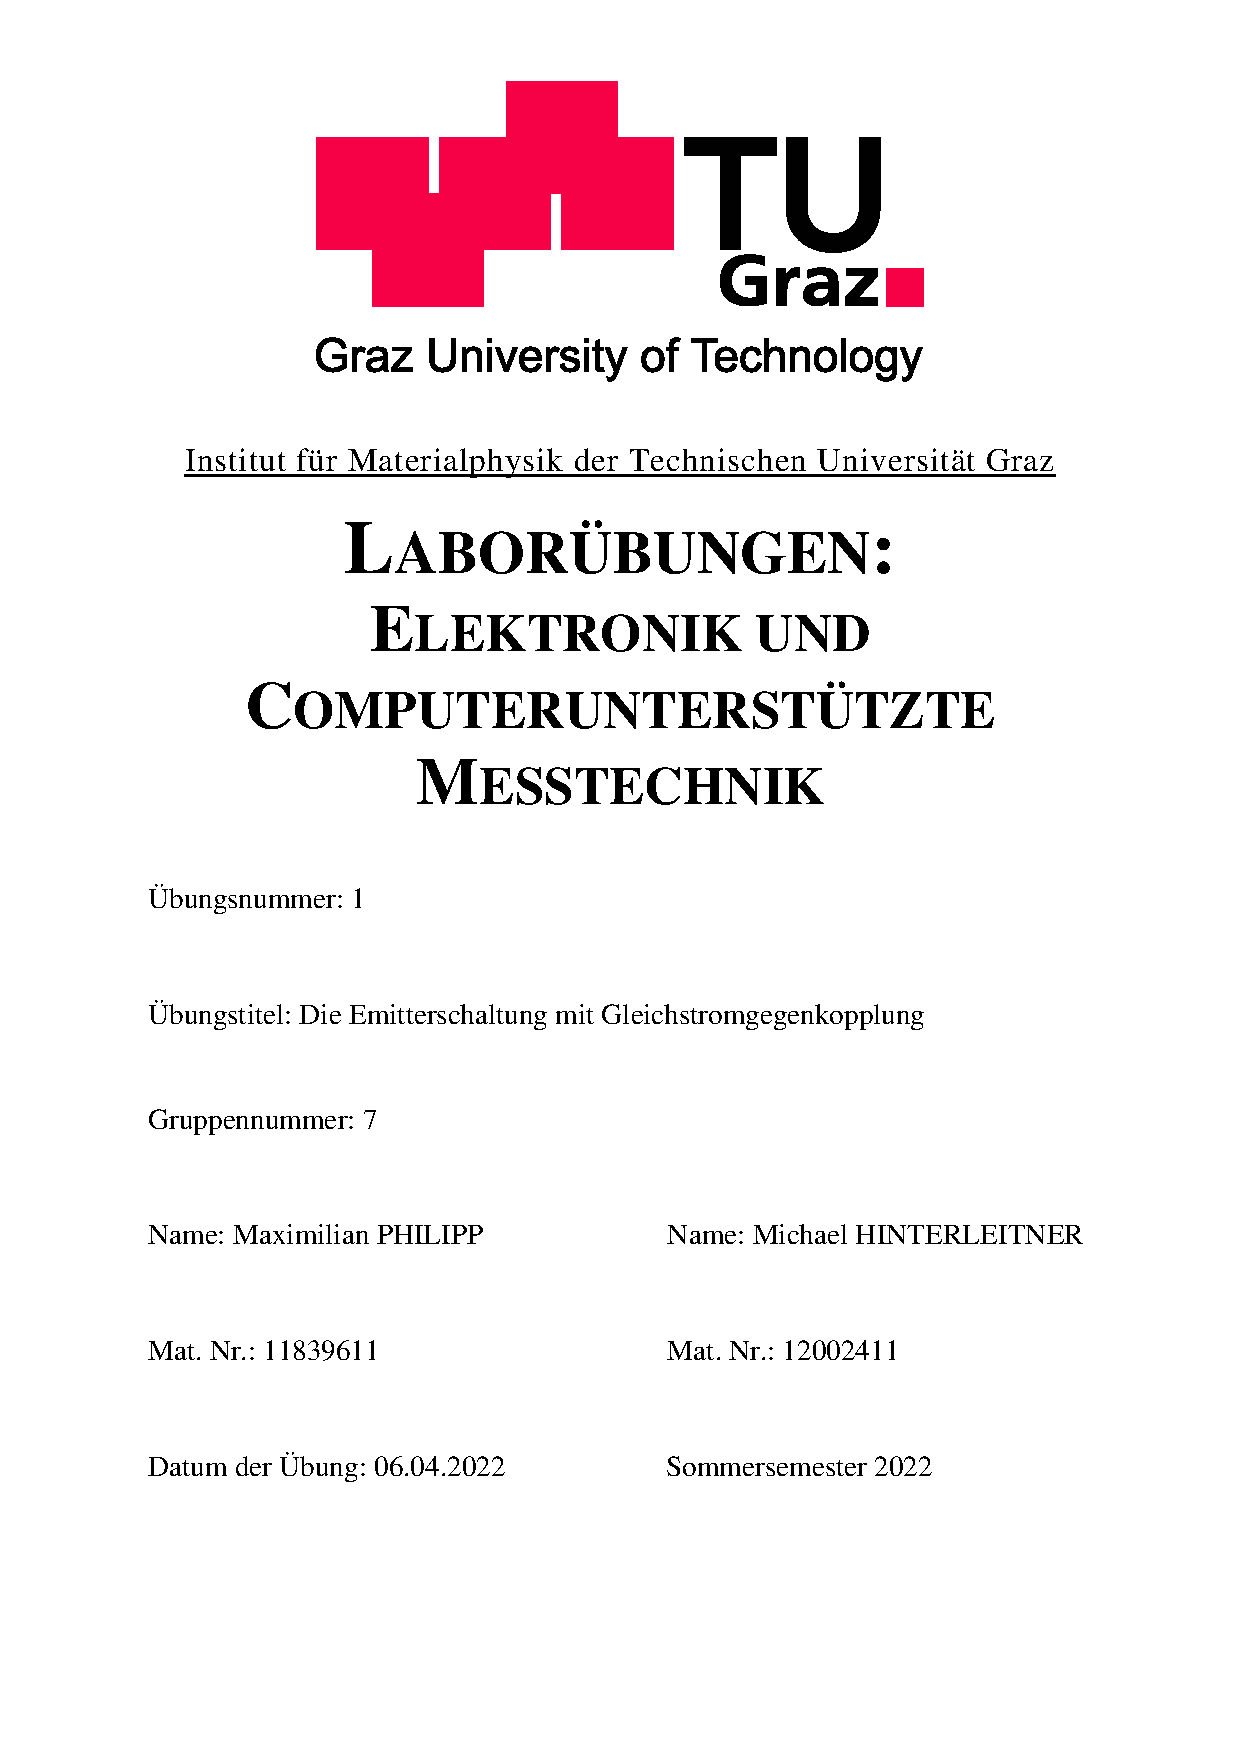
\includepdf{deckblatt1.pdf}
\tableofcontents
\newpage


% \section{Aufgabenstellung}\label{sec:Aufgabenstellung}

% Die nachfolgende Aufgabenstellung wurde von den Laborbetreuern bereitgestellt
% und beinhaltet sowohl Angaben zur Vorbereitung als auch zur praktischen
% Durchführung der Übung:

% zu 1: Aufgabenstellung Das vor der Übung verteilte Aufgabenblatt.
% TODO einkommentieren kompiliert schneller auskommentiert
% 
\includepdf[
%     pages=-,  % all pages
%     addtotoc={
%         1, section, 1, Aufgabenstellung, sec:aufgabenstellung
%     },
%     addtolist={
%        4, figure, {Ehemitverschaltung mit Gleichstromgegenkopplung}, fig:angabe_abb1,
%        4, figure, {Ersatzschaltbild Eingangs- und Ausgangswiderstand}, fig:angabe_abb2,
%        4, figure, {Ersatzschaltbild Koppelkondensatoren}, fig:angabe_abb3
%     }
% ]{angabe.pdf}

% zu 2: Vorbereitung Es sind beide Vorbereitungen dem Protokoll beizufügen.
\section{Vorbereitung}\label{sec:Vorbereitung}
%\includepdf[pages=-]{vorbereitung.pdf}
%TODO: einfügen der vorbereitung


% zu 3: Grundlagen In den Grundlagen sollen die später verwendeten Formeln
% stehen und kurz erklärt werden, dabei ist es nicht notwendig Formeln
% herzuleiten. Quellenangaben sind an dieser Stelle von Vorteil, weil Sie so
% schnell die betreffenden Stellen in Unterlagen finden. In den Rechnungen
% werden grundlegende Annahmen skizziert und begründet und dann mit diesen
% Annahmen, die für die Schaltungen notwendigen Werte berechnet. Dabei kann
% auch gleich auf die später wirklich verwendeten Werte Bezug genommen werden -
% wir verwenden bei den Widerständen zum Beispiel von den Normwert-Reihen die
% E12 und/oder E24 Serie (nach DIN 41426 bzw. IEC 63).
\section{Grundlagen}\label{sec:Grundlagen}

Bipolartransistoren sind Halbleiterbauelemente mit zwei pn-Halbleiterübergängen
(entweder npn oder pnp), bei denen gegensätzlich zu den Feldeffekttransistoren
beide Arten von Ladungsträgern, Elektronen und Löcher/Defektelektronen, am
Stromfluss beteiligt sind. Für Schaltungen mit Bipolartransistoren, die in der
Elektronik zur Verstärkung respektive Schaltung verwendet werden, wird zwischen
Emitter-, Basis- und Kollektorschaltung differenziert. Die
Schaltungsbezeichnungen beruhen auf dem Anschluss, der als Bezug für Eingang
und Ausgang dient. Diese Schaltungsarten sind in 
\autoref{fig:schaltungsarten} dargestellt; zu beachten ist, dass der Pfeil am
Emitter des Transistors in die technische Stromrichtung zeigt. 

\begin{figure}[H]
    \centering
    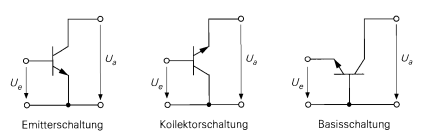
\includegraphics[width=8cm, height=8cm,keepaspectratio]{./figures/schaltungsarten.png}
    \caption{Darstellung der 3 Schaltungsarten mit Bipolartransistor \cite{tietze}}
    \label{fig:schaltungsarten}
\end{figure}

In dieser Laborübung sind ausschließlich Emitterschaltungen von Relevanz,
insbesondere jene mit Stromgegenkopplung, wodurch die Temperaturabhängigkeit
der Schaltung kompensiert wird. Dies ist deswegen von hoher Relevanz, da
Transistorschaltungen stets um einen bestimmten Arbeitspunkt betrieben werden
(sollten). Dieser Arbeitspunkt wird über den Kollektorstrom $I_C$, Basisstrom
$I_B$, der Kollektor-Emitterspannung $U_{CE}$ beziehungsweise
Basis-Emitterspannung $U_{BE}$ festgelegt. Ein Anstieg der Temperatur würde
diesen wiederum, aufgrund der Temperaturabhängigkeit von Halbleitern
(pn-Übergang), verschieben. Dadurch wird eine Zunahme des Basisstroms $I_B$ und
infolge des Kollektorstroms $I_C$ sowie eine Abnahme des Kollektorpotentials
$V_C$ bedingt. Um dies zu kompensieren, wird im Rahmen der Stromgegenkopplung
ein Emitterwiderstands $R_E$ implementiert. Dieser führt aufgrund des nun
höheren Emitterstroms $I_E$, der sich gemäß der Kirchhoff'schen Knotenregel aus
der Summe der Teilströme $I_C$ und $I_B$ (der allerdings vernachlässigt werden
kann) ergibt, zu einer größeren Spannung $U_{RE}$, die am Emitterwiderstand
abfällt. Dadurch nimmt die Basis-Emitterspannung $U_{BE}$ ab und der Basisstrom
wird geringer, genauso wie folglich der Kollektor- und Emitterstrom, was der
ursprünglichen Erhöhung entgegenwirkt. \cite{tietze}
\newline

Zur Berechnung der Ströme am Steckbrett (Kapitel \nameref{sec:Auswertung}), des
Basis- $I_B$ und Kollektorstroms $I_C$, nachdem die an den Vorwiderständen
$R_1$ und $R_2$ abfallenden Spannungen $U_{R1}$ respektive $U_{R2}$ gemessen
wurden, wird das Ohmsche Gesetz \autoref{eq:ohm} verwendet. Dabei bezeichnet
wie gewohnt $U$ die Spannung, $I$ den Strom und $R$ den Widerstand als die
Proportionalitätskonstante beziehungsweise für einen nicht-linearen Verlauf $r$
den differentiellen Widerstand an einem Arbeitspunkt. \cite{tietze}

\begin{align}
	R&=\frac{U}{I} \label{eq:ohm}\\
	r&= \der{U}{I} \Bigr|_{\substack{Arbeitspunkt}}
\end{align}

Die (Spannungs-)Verstärkung $V$ der Schaltung ergibt sich aus dem Verhältnis
zwischen Ausgangsspannung und Eingangsspannung gemäß \autoref{eq:verst}.

\begin{equation}
	V=\frac{U_a}{U_e}
	\label{eq:verst}
\end{equation}

% zu 4: Versuchsdurchführung In diesem Punkt wird die Durchführung der
% einzelnen Aufgaben beschrieben. Im Simulationsteil ist die simulierte
% Schaltung mit allen Analyseparametern darzustellen. Im praktischen Teil sind
% die verwendete Geräte sowie die gemessenen Werte der verwendeten Bauteile
% anzugeben. Außerdem sind durchgeführte Funktionsüberprüfungen der Bauteile
% (Dioden, Transistor, etc.) anzuführen. Die Messergebnisse bzw. Oszillogramme
% sind mit Angabe der verwendeten Messgeräte anzugeben. Oszillogramme werden
% vom verwendeten Oszilloskop als Daten auf einen USB-Stick ausgegeben und
% können in das Protokoll aufgenommen werden. Das gleiche gilt für Schaltungen
% bzw. Ergebnissen von Simulationen. Es ist auf eine klare Darstellung der
% Messergebnisse und –auswertung zu achten (Tabellen, geeignete Grafiken). Die
% originalen, während des Versuchs angefertigten Aufzeichnungen sind dem
% Protokoll beizufügen. 
\section{Versuchsdurchführung}\label{sec:Versuchsdurchf}

\subsection{Simulation} \label{sec:Versuchsim}

Zur Simulation der Emitterschaltung mit Gegenstromkopplung wird das Programm
\textit{LTSPICE} verwendet. Der Aufbau erfolgt analog zum skizzierten Schaltplan im
Kapitel \nameref{sec:Vorbereitung}. 

% DONE 1.1 Bauen Sie die Schaltung mit dem Programm PSPICE LT gemäß der berechneten
% DONE Parameter ohne den Überbrückungskondensator CE auf.
\subsubsection{Schaltung ohne Überbrückungskondensator} \label{sec:Versuchohnekond}

Zunächst wird die Schaltung allerdings ohne Überbrückungskondensator, wie sie
in  \autoref{fig:schaltungohnekond} zu sehen ist, verwendet. Nachdem
alle Parameter gemäß den Angaben in der Simulation und insbesondere der
Arbeitspunkt entsprechend dem theoretisch errechneten Wert eingestellt wurden
(ca. \SI{7.5}{\volt}), wurden die Eingangs- und Ausgangsspannung über der Zeit in
einem Plot, durch Messung dieser Größen für einen geeigneten Zeitabschnitt
(siehe  \autoref{fig:schaltungohnekond} im unteren Bildbereich),
dargestellt. 

\begin{figure}[H]
    \centering
    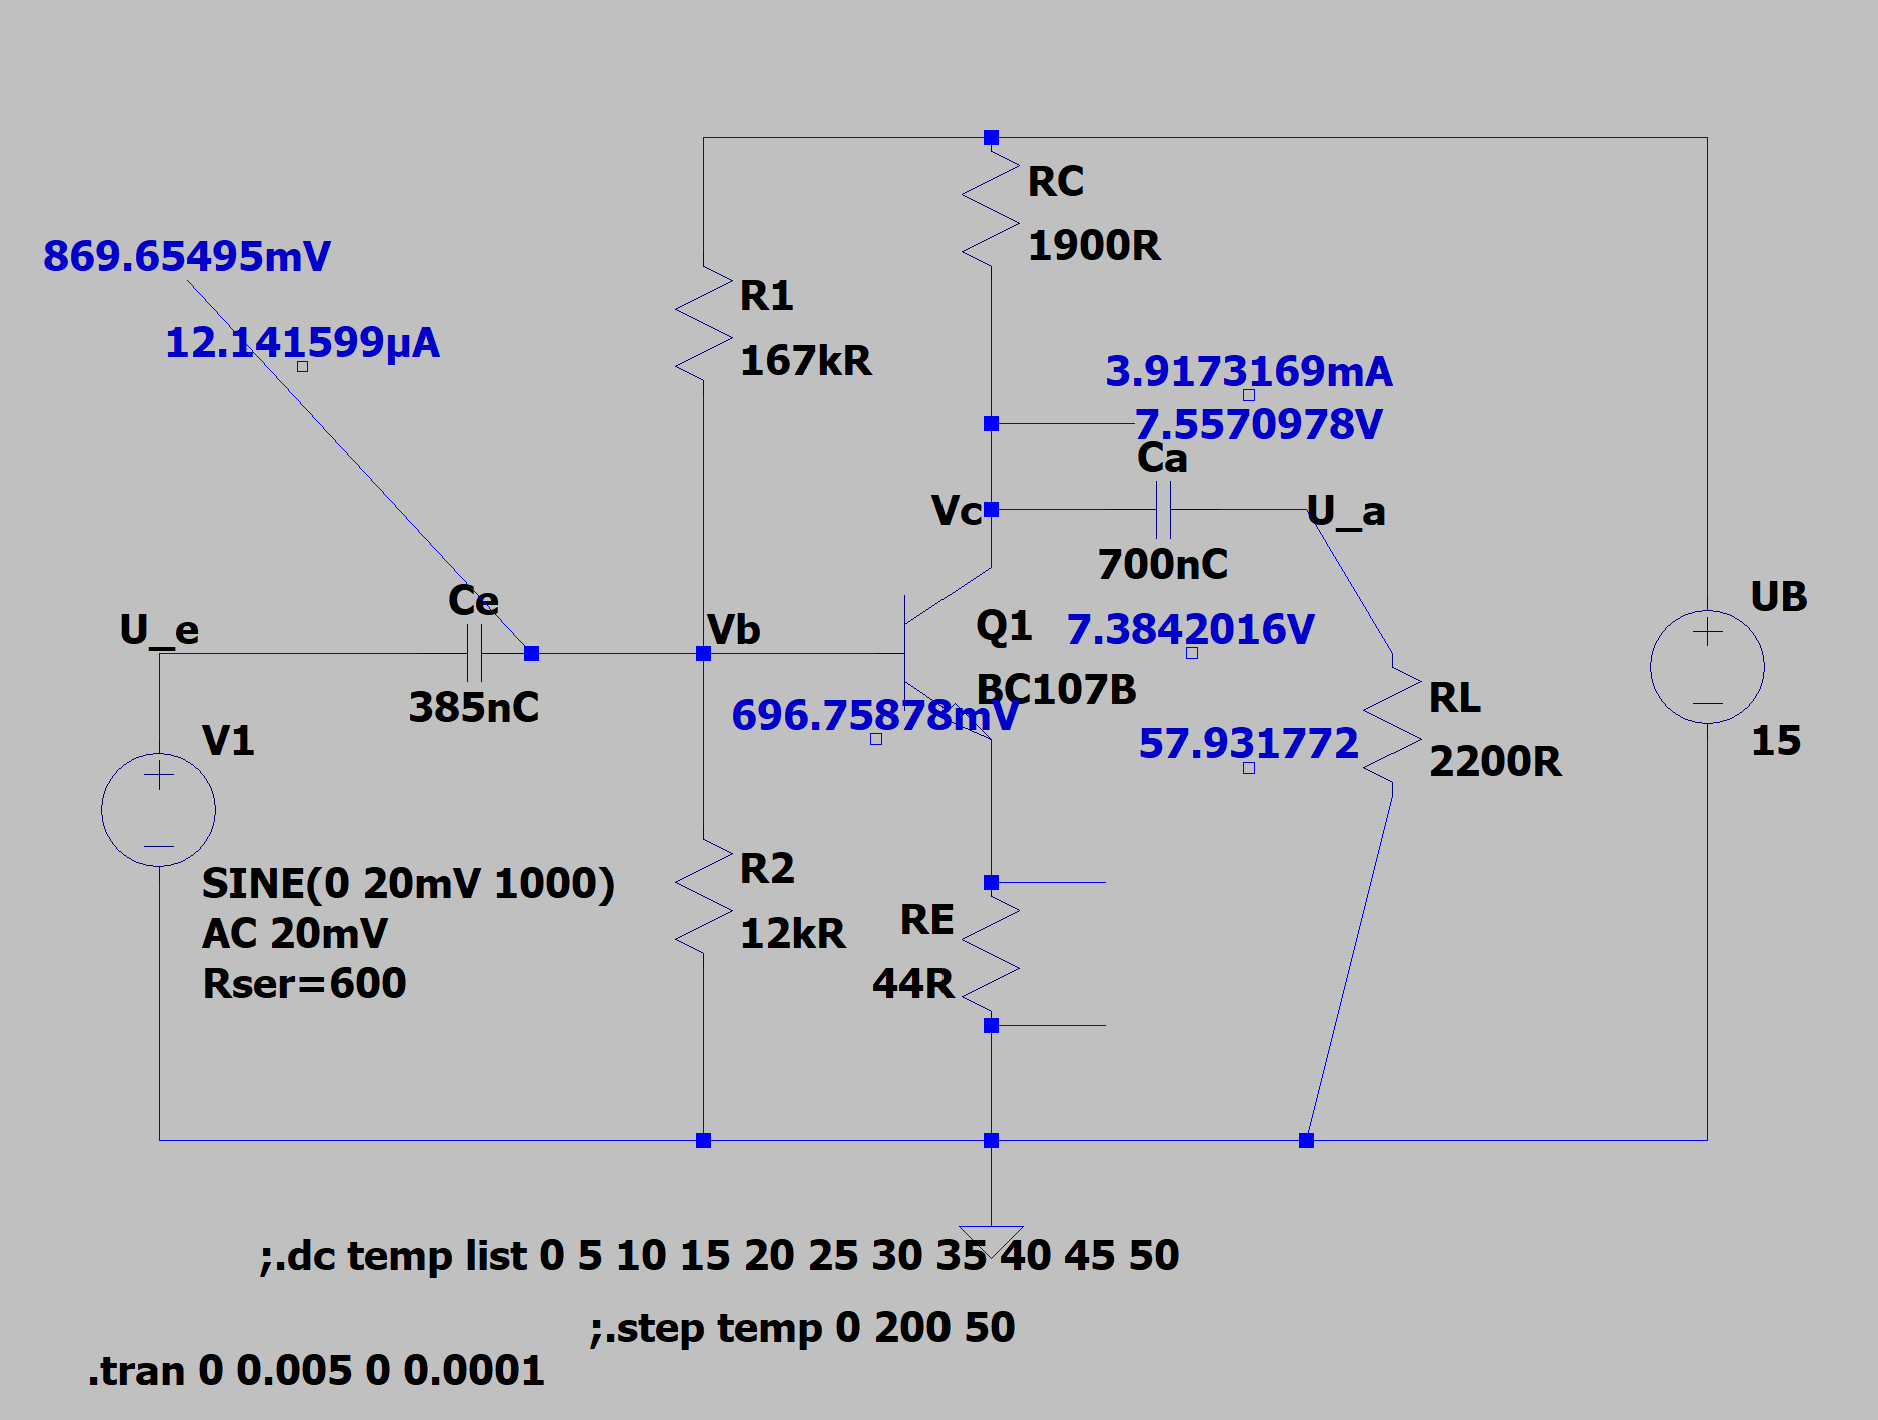
\includegraphics[width=8cm, height=8cm,keepaspectratio]{./figures/ohnekond/schaltungmitmessungen20mv.png}
    \caption{Schaltung ohne Überbrückungskondensator bei einem Sinus-Eingangssignal
    mit einer Amplitude von \SI{20}{mV}, einer Frequenz von \SI{1}{k\hertz} und einem
    Innenwiderstand von \SI{600}{\ohm} ; mit der Eingangs- $U_e$ und
    Ausgangsspannung $U_a$, den Eingangs- $Ce$ und Ausgangskondensatoren $Ca$, den
    Vorwiderständen $R1$ und $R2$, dem Kollektorwiderstand $RC$, dem
    Emitterwiderstand $RE$, dem Lastwiderstand $RL$, dem Basispotential $Vb$, dem
    Kollektorpotential $Vc$, dem Transistor \textit{BC107B} und der
    Betriebsspannung $UB$. Genauere Spezifikationen können dem Schaltbild entnommen
    werden.}
    \label{fig:schaltungohnekond}
\end{figure}

% FIXME(MAX) 1.2 Stellen Sie eine Eingangs-Sinusspannung von 1 kHz mit einer Amplitude innerhalb der
% FIXME(MAX) Übersteuerungstoleranzen ein, erzeugen Sie ein Simulation Profil (Time Domain) und nehmen Sie
% FIXME(MAX) jeweils die Eingangsspannung und die Ausgangsspannung in einem Plot über die Zeit auf. Lassen Sie
% FIXME(MAX) sich auch die Spannungen und Ströme im Schaltbild anzeigen 
% um den Arbeitspunkt diskutieren zu
% können. Berechnen Sie daraus die simulierte Verstärkung und diskutieren Sie die beiden Diagramme
% und ihren Zusammenhang.

\paragraph{Normalbetrieb}

In \autoref{fig:verlaufohnekond} ist der zeitliche Verlauf von Eingangs-
und Ausgangsspannung der Emitterschaltung ohne Überbrückungskondensator
dargestellt.

\begin{figure}[H]
    \centering
    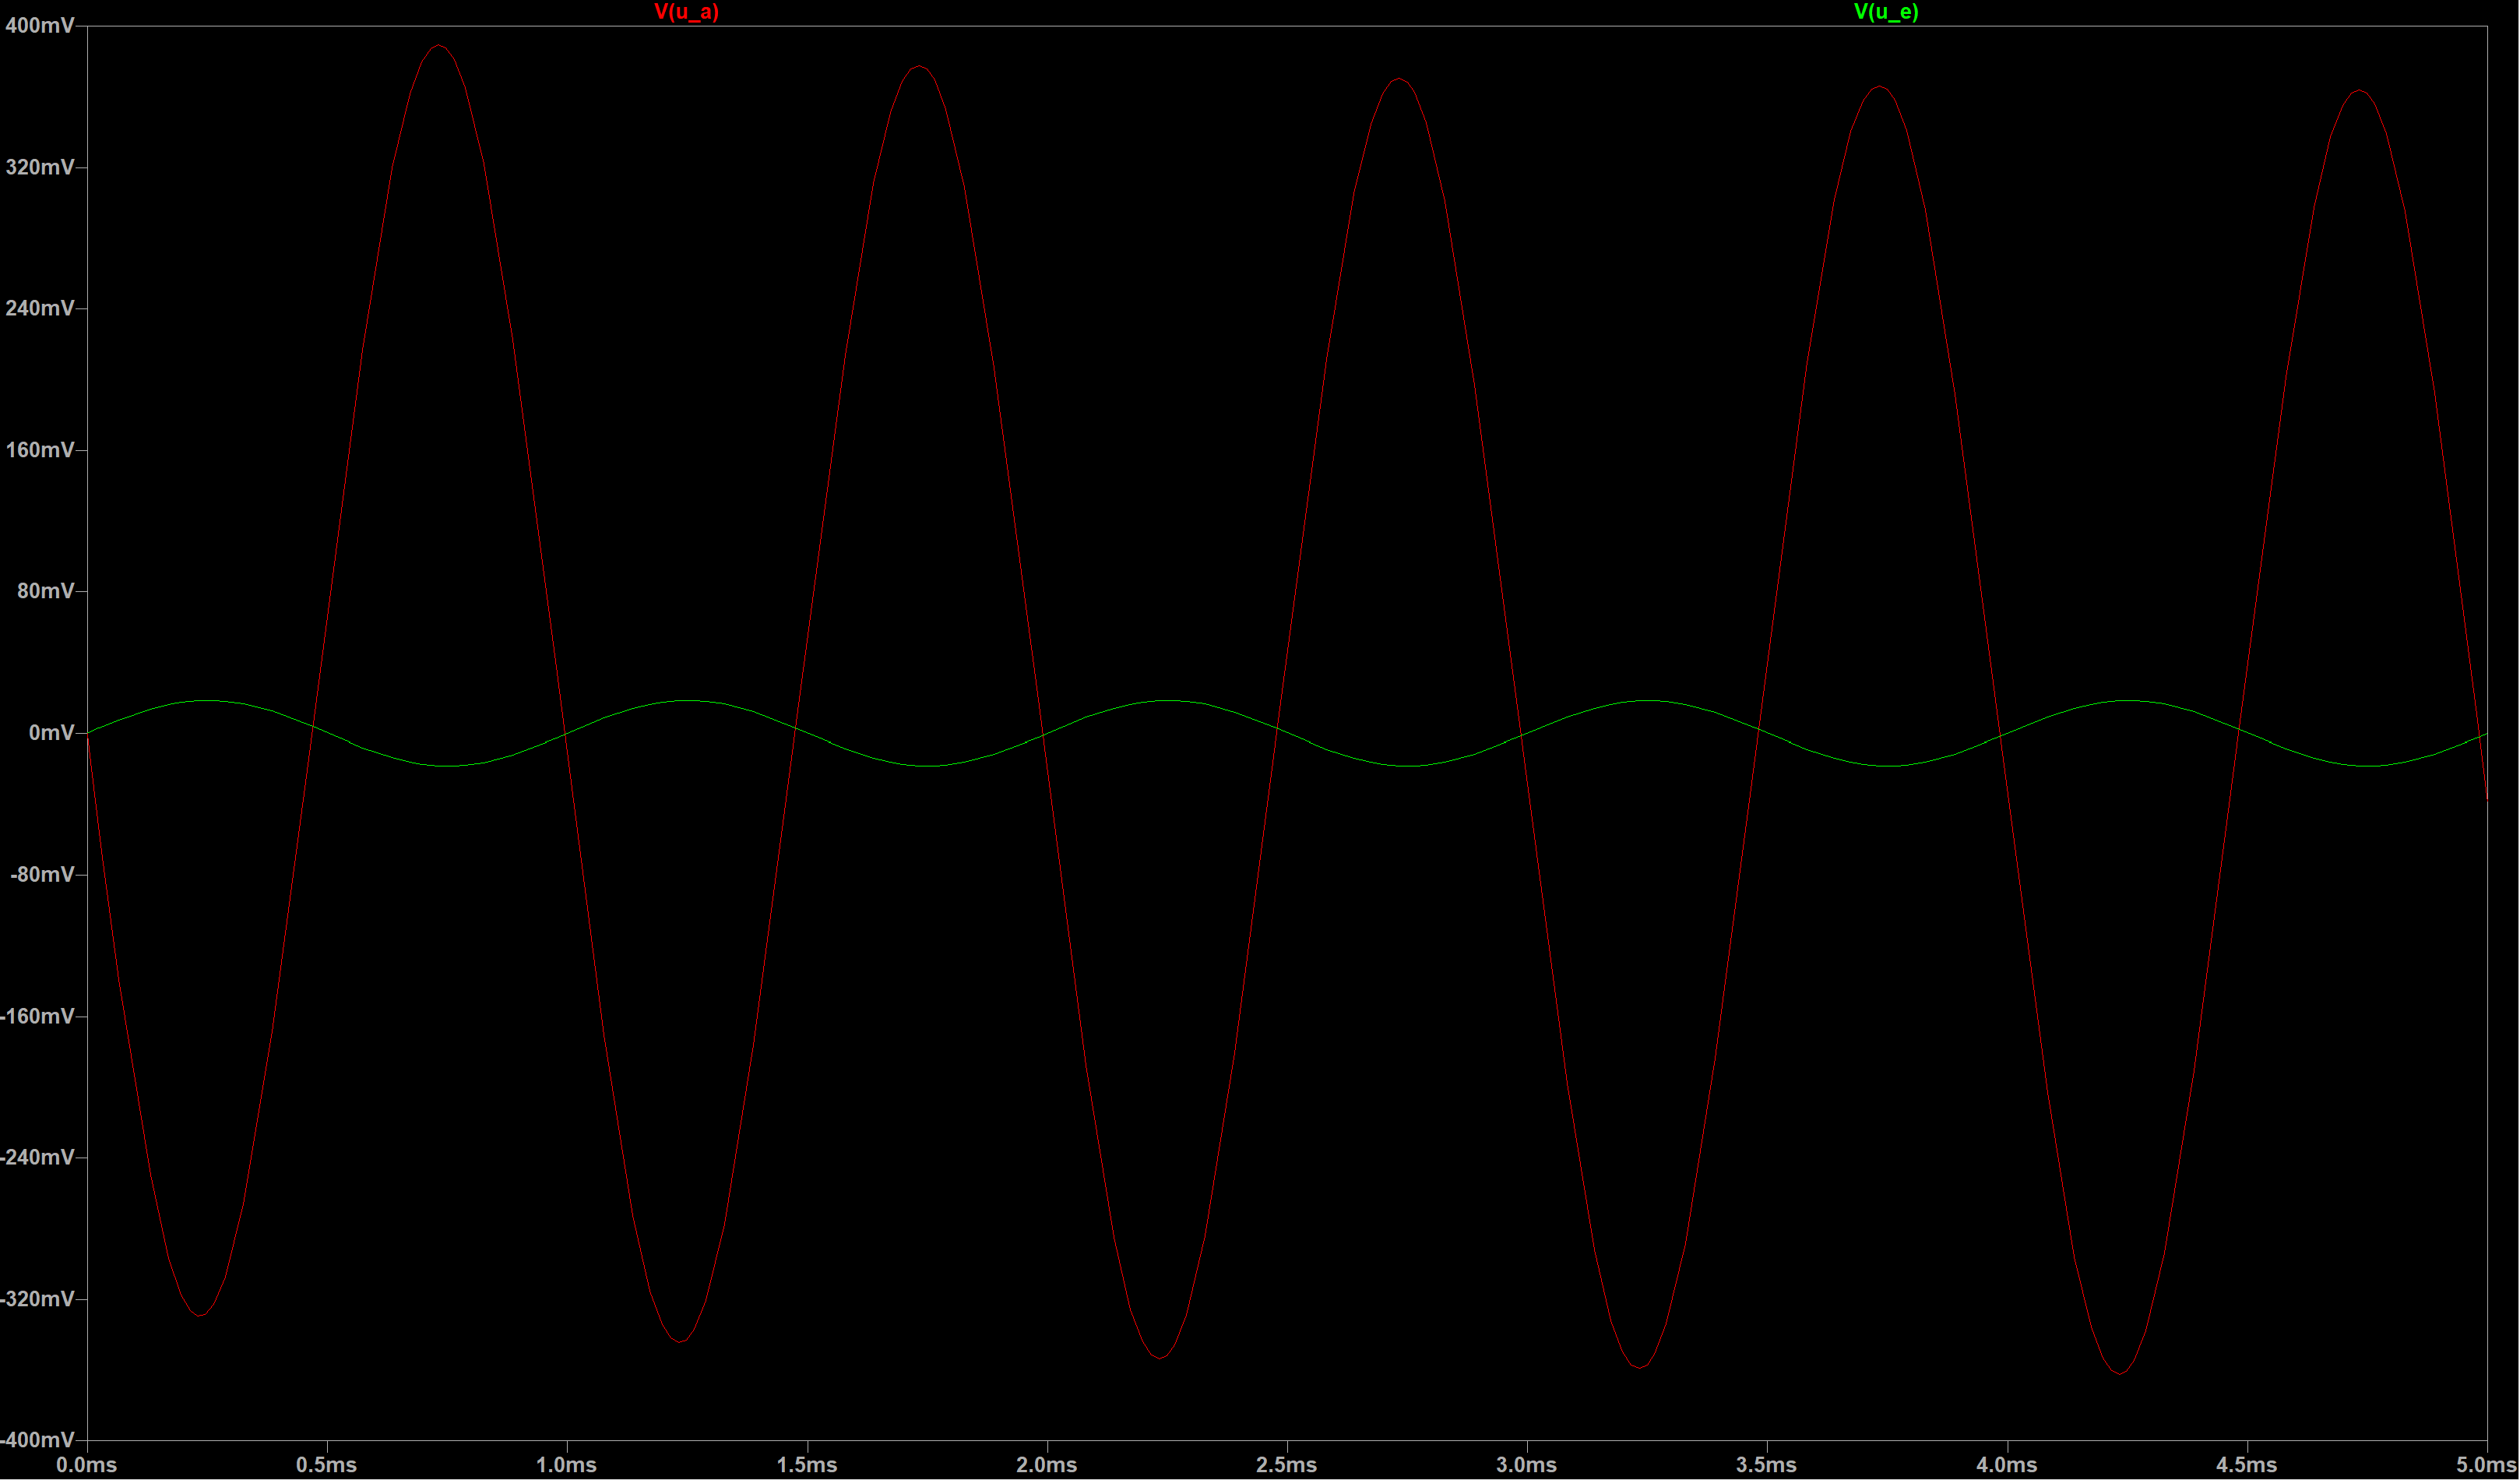
\includegraphics[width=\linewidth, height=7cm]{./figures/ohnekond/eingangundausgangssignal.png}
    \caption{Zeitlicher Verlauf der Ein- $V(u_e)$ und Ausgangsspannung $V(u_a)$
    der Emitterschaltung ohne Überbrückungskondensator bei einer Amplitude von
    \SI{20}{mV} des Eingangssignals}
    \label{fig:verlaufohnekond}
\end{figure}

% FIXME(MAX) 1.3 Testen Sie wie hoch die maximale Eingangspannung werden darf bis der Transistor in der Simulation
% FIXME(MAX) übersteuert. Übersteuern Sie ihn anschließend und nehmen Sie wieder die Eingangspannung sowie
% FIXME(MAX) die Ausgangsspannung nach der Zeit auf 
% und diskutieren Sie anhand dieses Plots die auftretenden
% Verzerrungen.

\paragraph{Übersteuerungsbetrieb}

% TODO erstellen eines Parametersweep um die Übersteuerungsgrenze gut darzustellen
Um die Übersteuerungsgrenze zu finden, wurde ein Parameter-Sweep durchgeführt,
wobei die Amplitude der Eingangsspannung variiert wurde. Dadurch konnte die
Übersteuerungsgrenze visuell bestimmt werden.



% FIXME(MAX) 1.4 Erstellen Sie einen DC Sweep in Abhängigkeit der Temperatur und zeigen Sie die Änderung des
% FIXME(MAX) Kollektorpotentials. 
% Diskutieren Sie die Konsequenzen einer Temperaturerhöhung.
\paragraph{DC Temperatur Sweep}
%TODO der text
Zur Darstellung der Temperaturabhängigkeit wurde ein DC-Sweep durchgeführt. In \autoref{fig:sim_dc_temp_sweep_ohne} ist das Kollektorpotential in Abhängigkeit der Temperatur zu sehen.
% TODO verbessere mich
\begin{figure}[H]
  \centering
    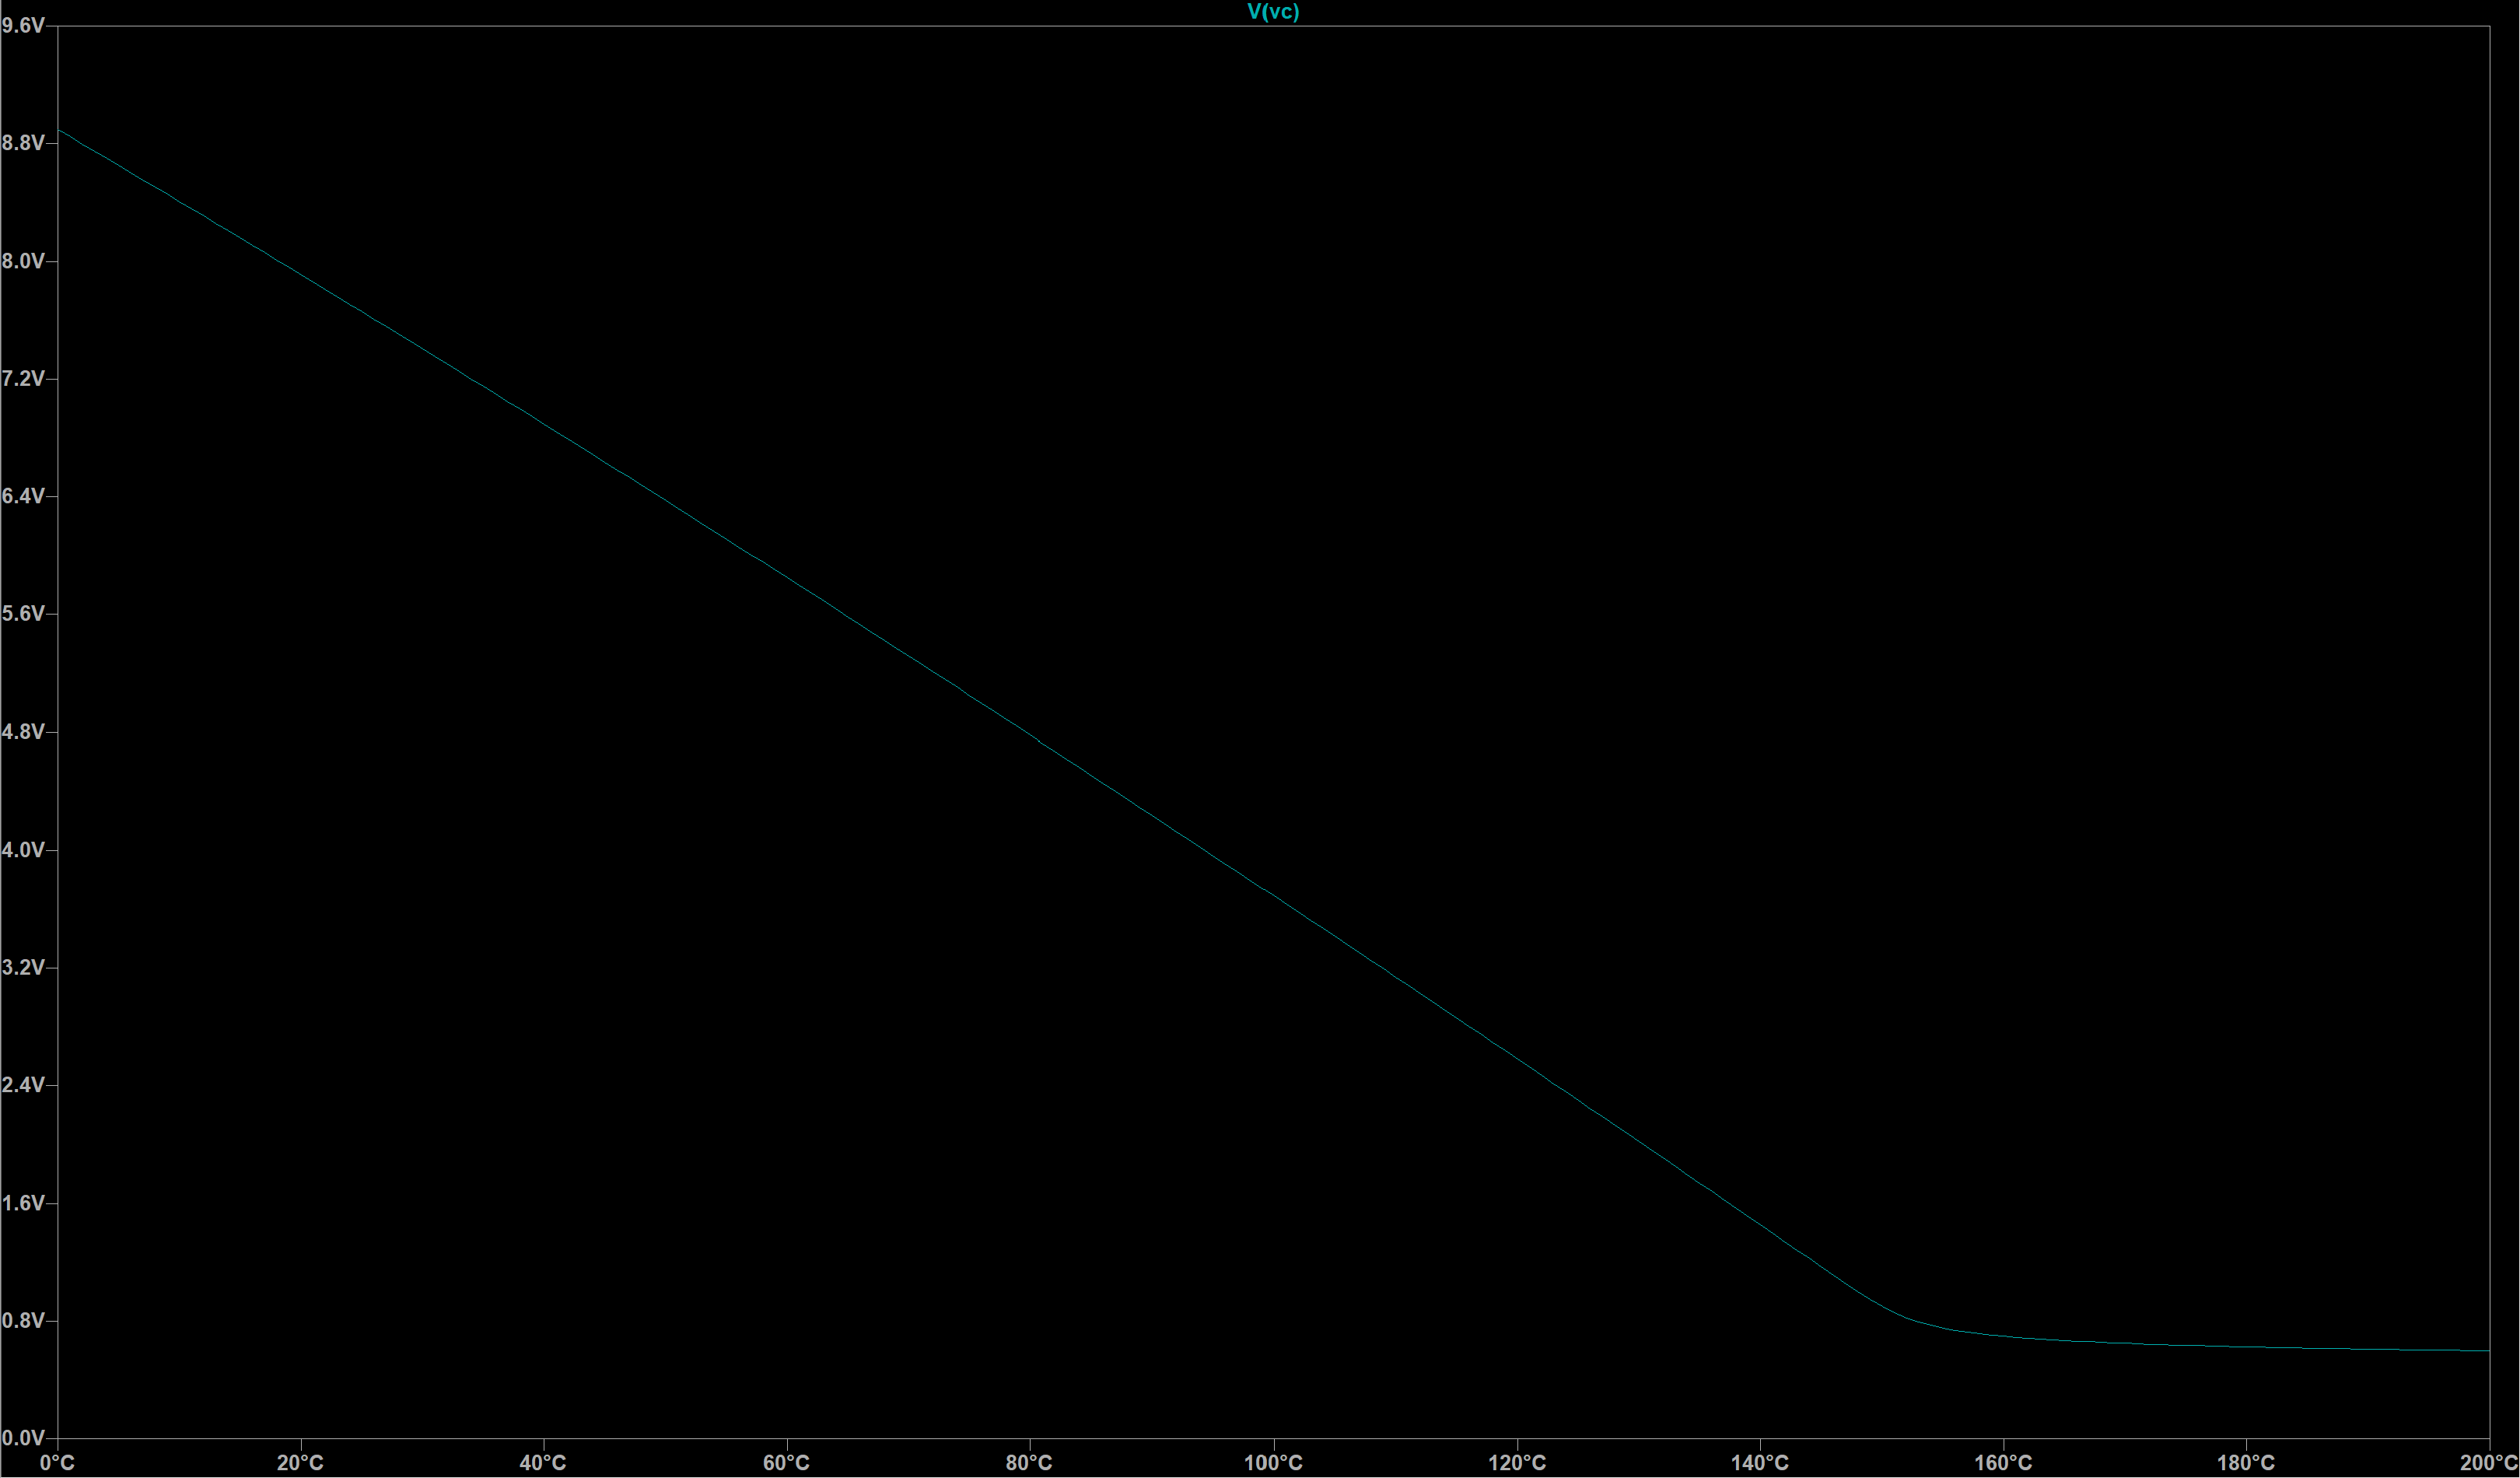
\includegraphics[width=\linewidth, height=7cm]{./figures/ohnekond/tempsweepdclinear.png }
    % TODO verbessere mich und ueberpruefe spice directive
    \caption[Simulierter DC Temperatur Sweep ohne
    Überbrückungskondensator]{Simulierter DC Temperatur Sweep welcher die
      Temperaturabhängigkeit des Kollektorpotentials darstellt. Auf der
      Abszisse befindet sich die Temperatur des Transistors und auf Ordinate
      befindet sich das Kollektorpotential $VC$. Diese Simulation wurde bei dem
      Schaltplan aus \autoref{fig:schaltungohnekond} mit folgender SPICE
      directive \texttt{.dc temp 0 200 1} durchgeführt.
  }
  \label{fig:sim_dc_temp_sweep_ohne}
\end{figure}


% 1.5 Nehmen Sie die Ausgangsspannung über der Zeit für verschiedene Temperaturen in einem
% Diagramm dar und diskutieren Sie diesen Plot.
\paragraph{Temperaturvariierte Transiente Analyse}
%TODO der text
Für die Ausgangsspannung wurde eine temparaturvariierte, transiente Analyse durchgeführt. Für fünf verschiedene Betriebstemperaturen ist der Verlauf der Ausgangsspannung in \autoref{fig:sim_tran_temp_ohne} zu sehen.

\begin{figure}[H]
  \centering
    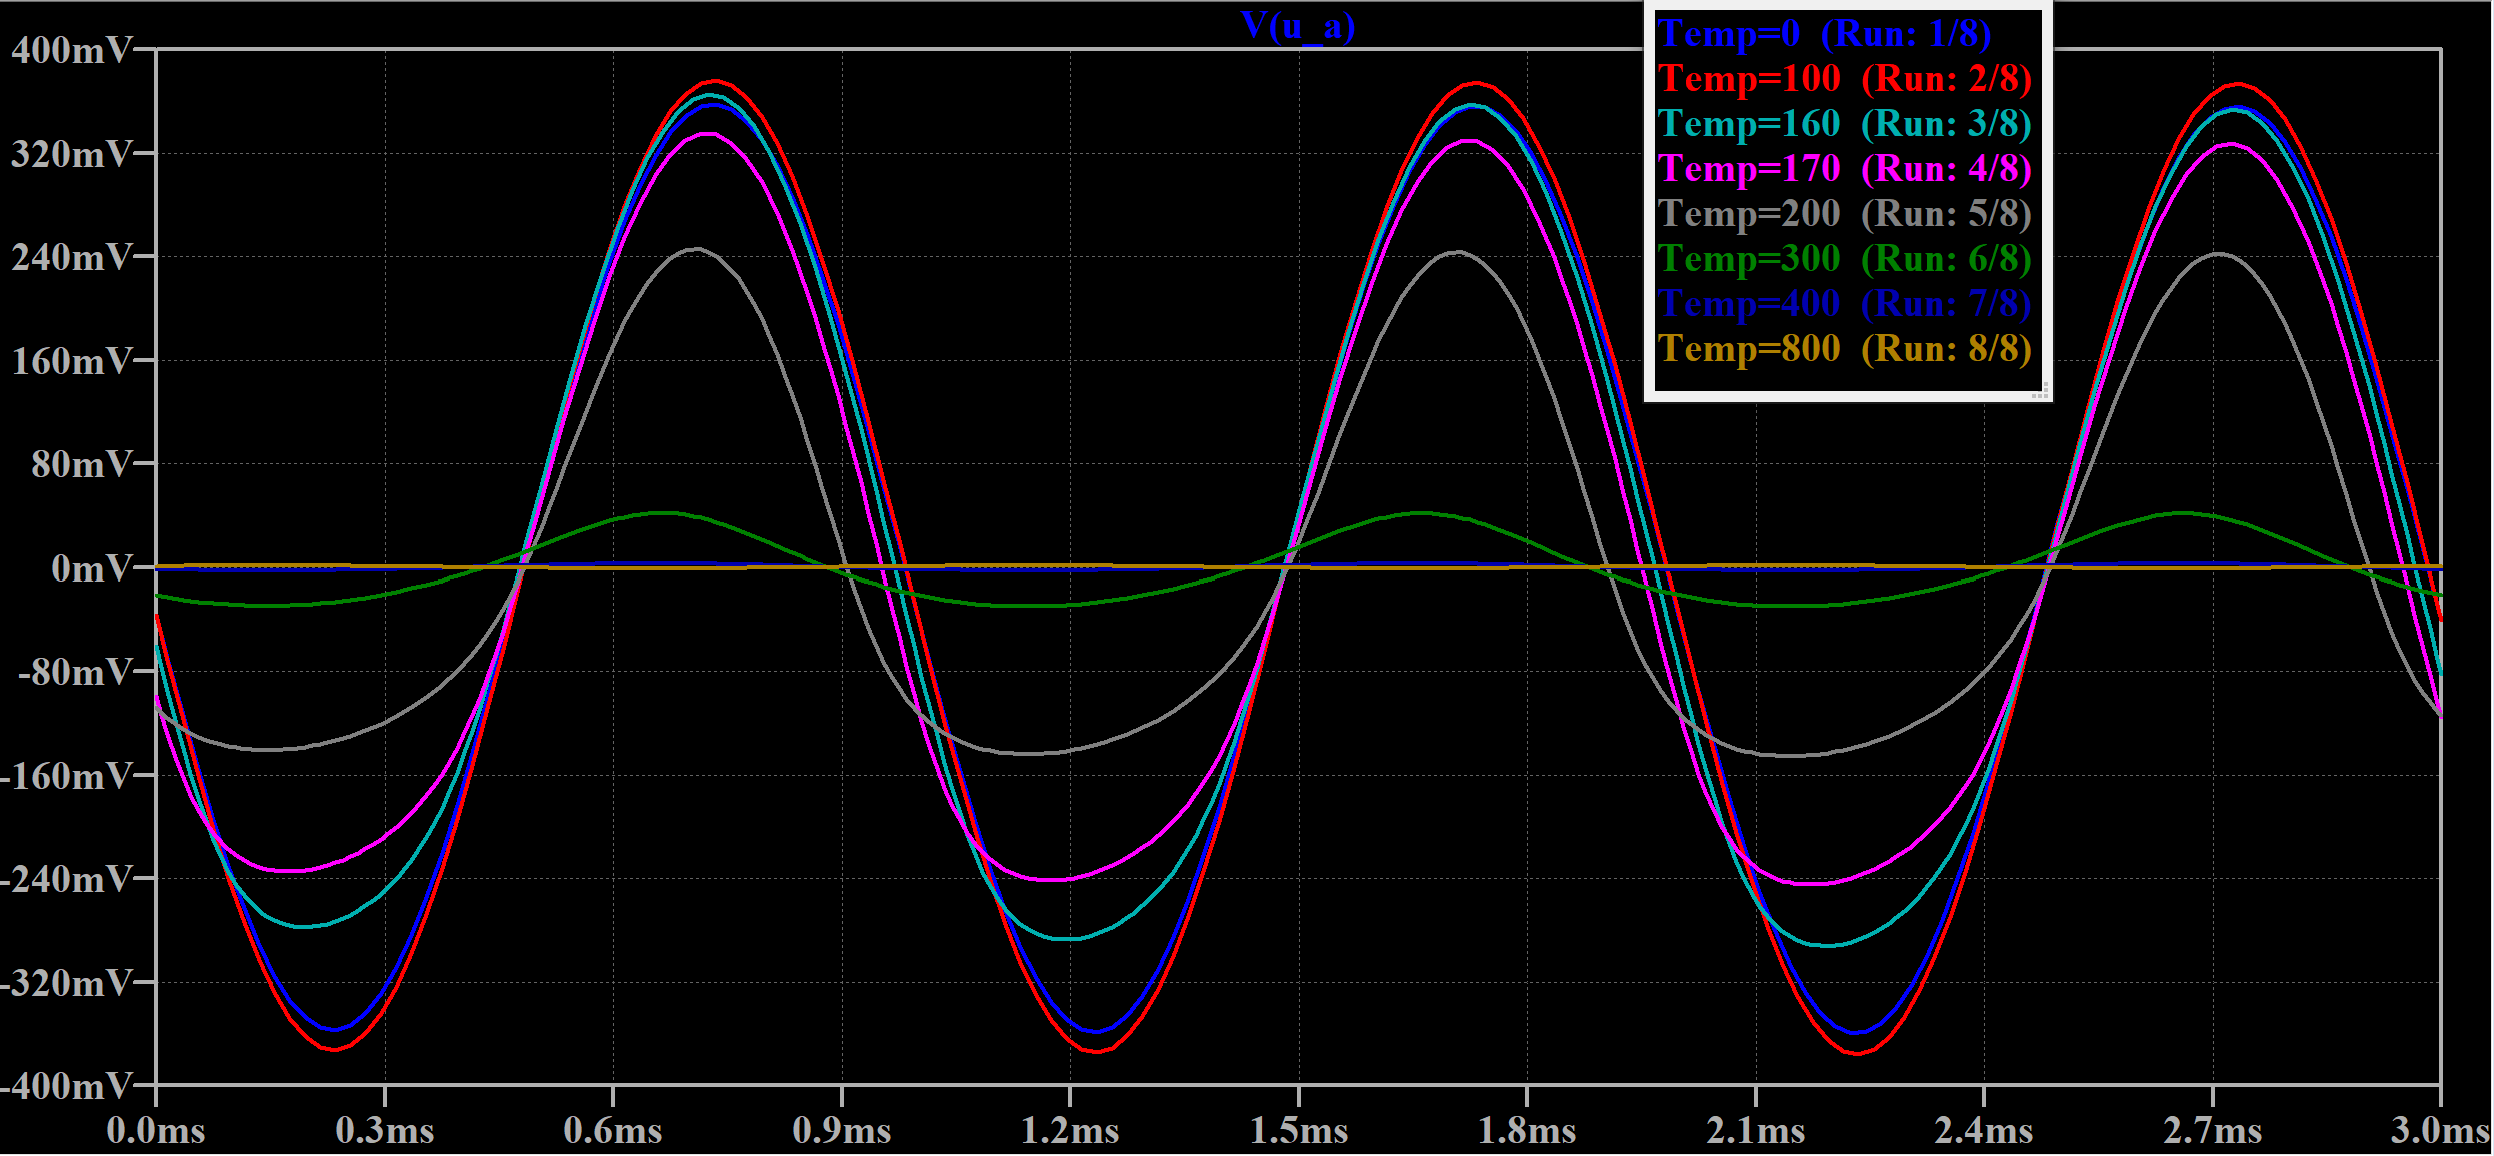
\includegraphics[width=\linewidth, height=7cm]{./figures/ohnekond/tempsweepausgang.png }
    % TODO verbessere mich und ueberpruefe spice directive
    \caption[Simulierte Transient Analyse ohne
    Überbrückungskondensator]{Simulierte Transient Analyse von der
      Ausgangsspannung unter Einfluß verschiedener Betriebstemperaturen. Auf
      der Abszisse befindet sich die Zeit und auf Ordinate befindet sich die
      Ausgangsspannung $U_a$. Diese Simulation wurde bei dem Schaltplan aus
    \autoref{fig:schaltungohnekond} mit folgenden SPICE directives \texttt{.tran
      0 0.005 0 0.0001} und \texttt{.step temp 0 200 50} durchgeführt. Die Legende
    beinhaltet die Zuordnung von Farbe zu Temperatur (in Celsius).}
  \label{fig:sim_tran_temp_ohne}
\end{figure}


% 2.1 Bauen Sie nun den Überbrückungskondensator CE ein. Verfahren Sie wie bei 1.2 bis 1.5.
\subsubsection{Schaltung mit Überbrückungskondensator} \label{sec:Schaltung mit Überbückungskondensator}

Nun wird die Schaltung der  \autoref{fig:schaltungohnekond} um den
Überbrückungskondensator $C_E$ gemäß  \autoref{fig:schaltungmitkond}
erweitert. Nun werden die gleichen Schritte wie beim vorigen Aufbau
durchlaufen.

\begin{figure}[H]
    \centering
    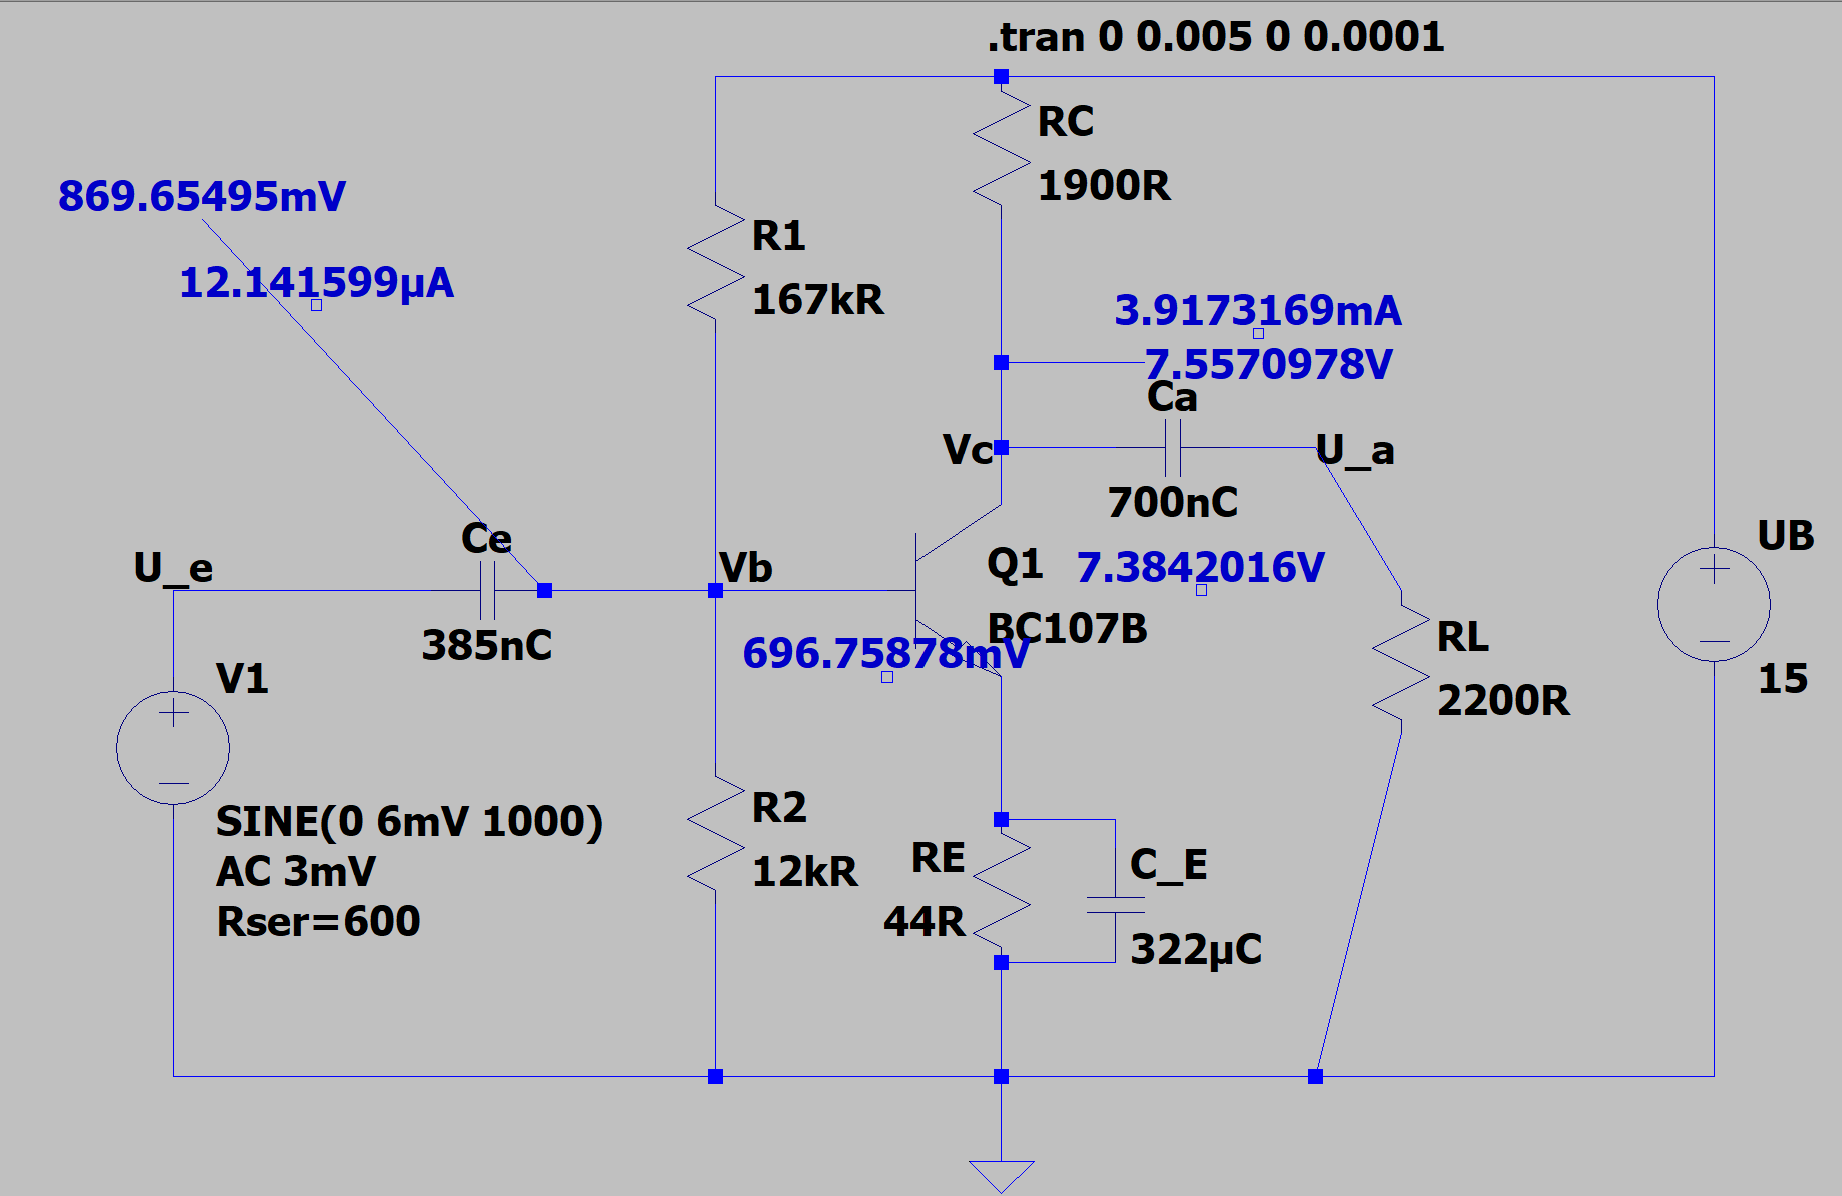
\includegraphics[width=8cm, height=8cm,keepaspectratio]{./figures/mitkond/messwertemitueberbrueckung.png}
    \caption{Schaltung mit Überbrückungskondensator bei einem Sinus-Eingangssignal
    mit einer Amplitude von \SI{6}{\milli\volt}, einer Frequenz von \SI{1}{\kilo\hertz} und einem
    Innenwiderstand von \SI{600}{\ohm} ; mit der Eingangs- $U_e$ und
    Ausgangsspannung $U_a$, den Eingangs- $Ce$ und Ausgangskondensatoren $Ca$, den
    Vorwiderständen $R1$ und $R2$, dem Kollektorwiderstand $RC$, dem
    Emitterwiderstand $RE$, dem Lastwiderstand $RL$, dem Basispotential $Vb$, dem
    Kollektorpotential $Vc$, dem Transistor \textit{BC107B} und der
    Betriebsspannung $UB$. Genauere Spezifikationen können dem Schaltbild entnommen
    werden.}
    \label{fig:schaltungmitkond}
\end{figure}

% FIXME(MAX) 2.2 Stellen Sie eine Eingangs-Sinusspannung von 1 kHz mit einer Amplitude innerhalb der
% FIXME(MAX) Übersteuerungstoleranzen ein, erzeugen Sie ein Simulation Profil (Time Domain) und nehmen Sie
% FIXME(MAX) jeweils die Eingangsspannung und die Ausgangsspannung in einem Plot über die Zeit auf. Lassen Sie
% FIXME(MAX) sich auch die Spannungen und Ströme im Schaltbild anzeigen 
% um den Arbeitspunkt diskutieren zu
% können. Berechnen Sie daraus die simulierte Verstärkung und diskutieren Sie die beiden Diagramme
% und ihren Zusammenhang.
\paragraph{Normalbetrieb}

Die Ein- und Ausgangsspannungen der Emitterschaltung mit
Überbrückungskondensator über der Zeit sind in \autoref{fig:sim_mit_normal_eingang} und \autoref{fig:sim_mit_normal_ausgang}
ersichtlich.

\begin{figure}[H]
    \centering
    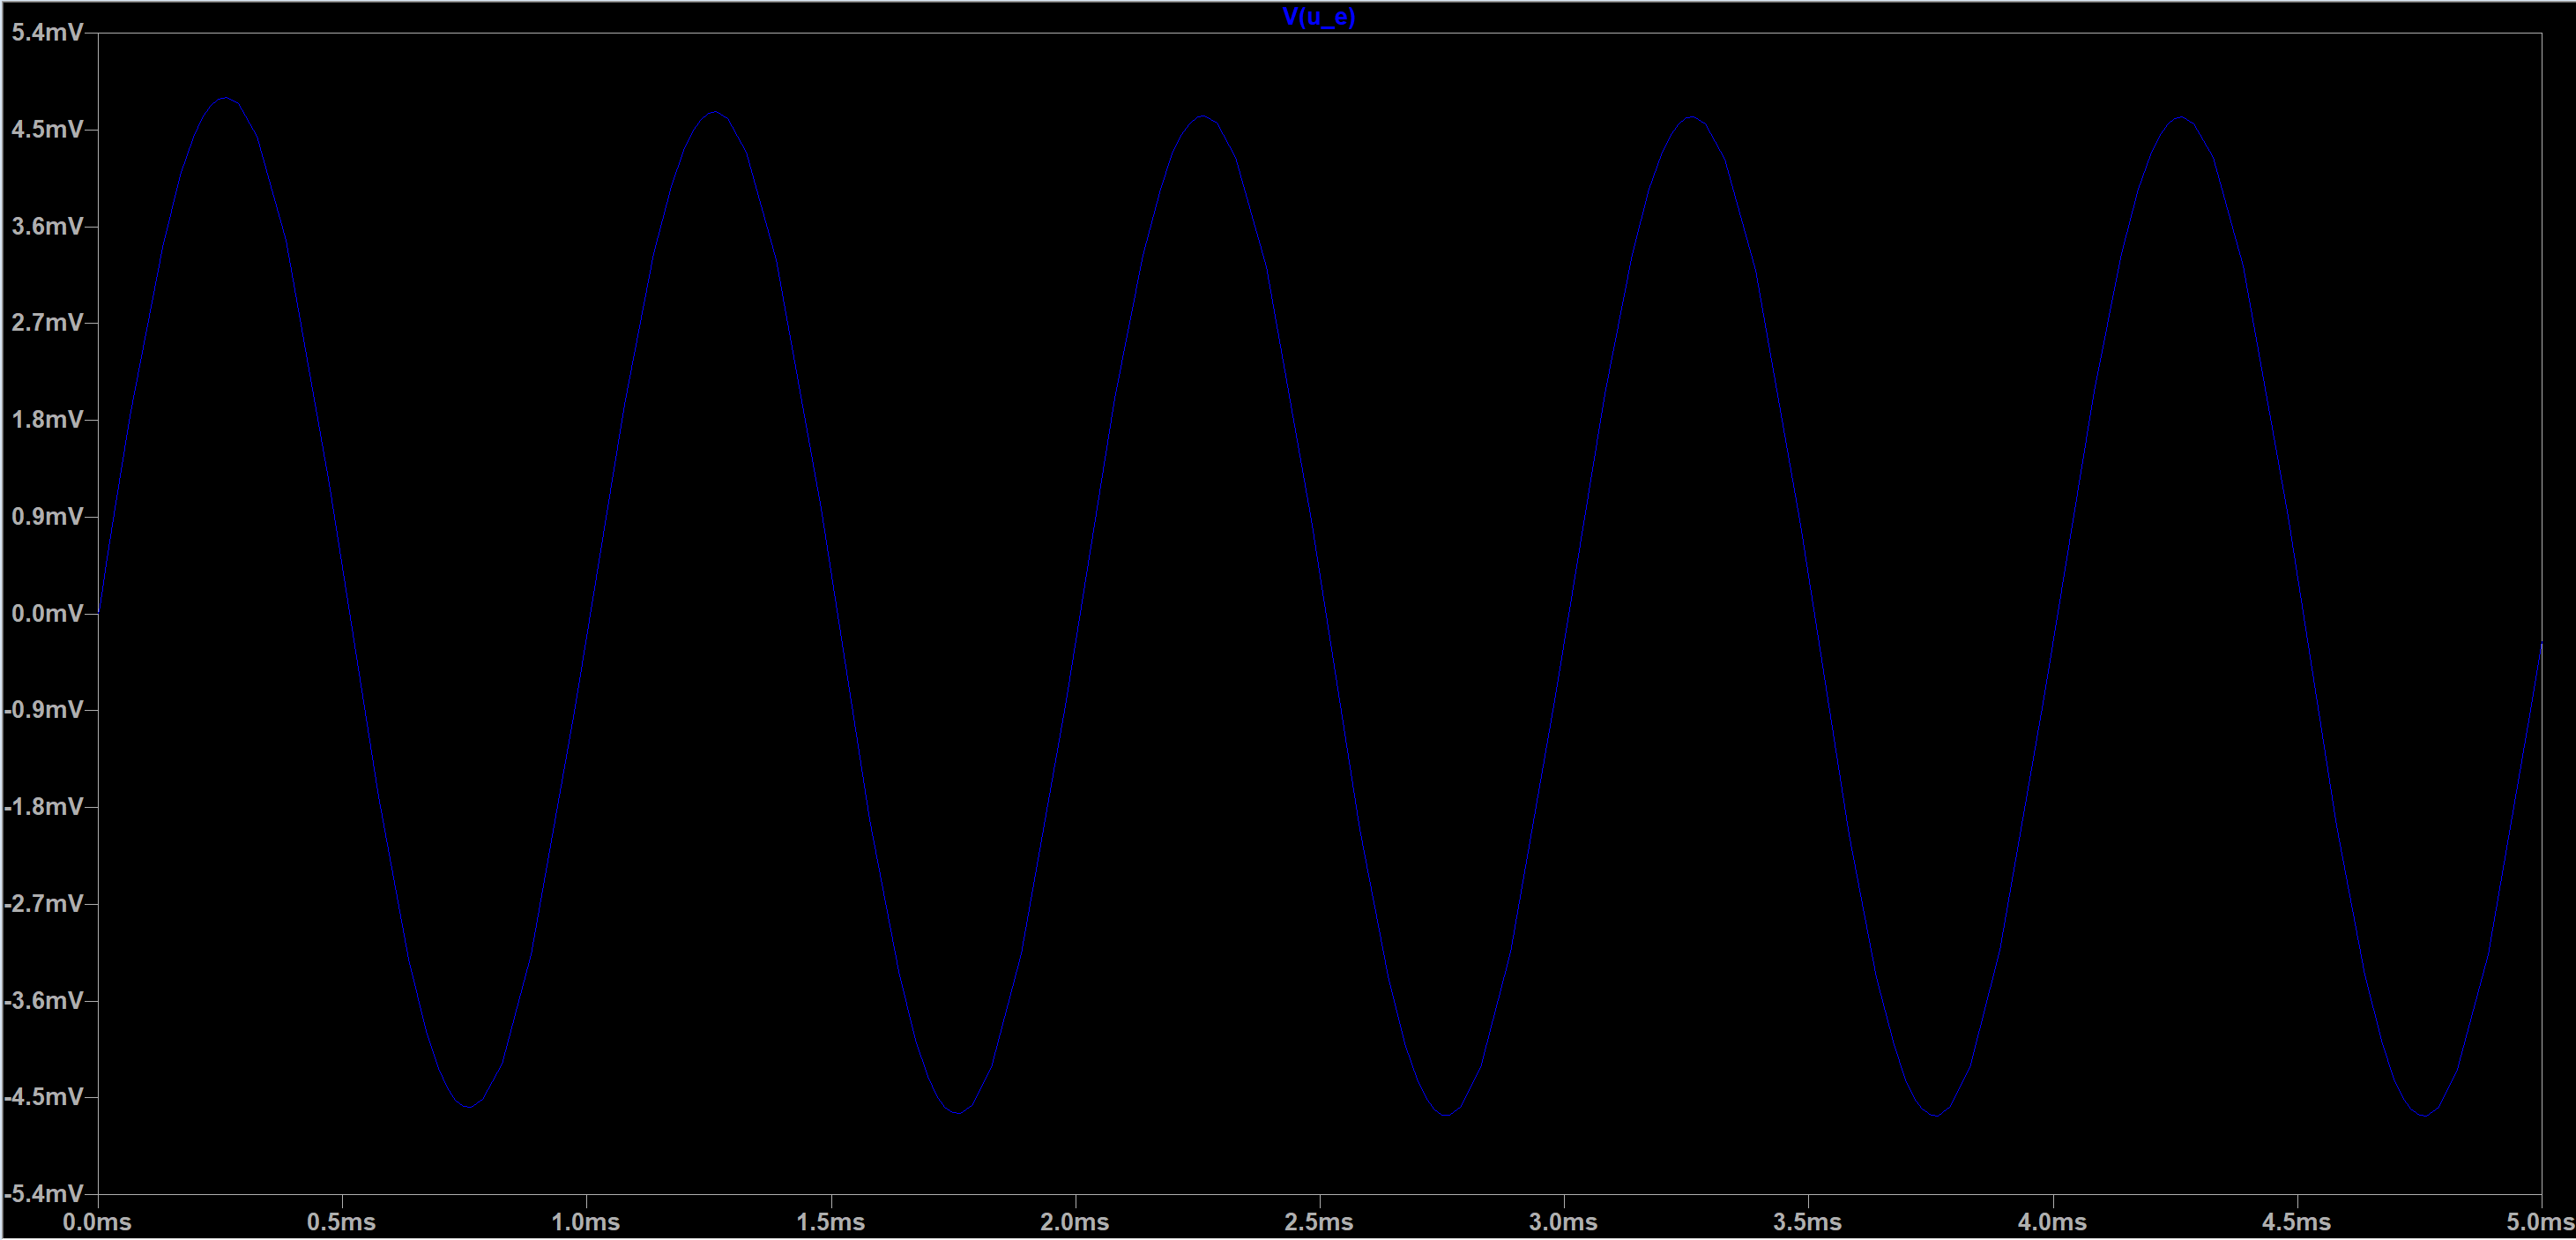
\includegraphics[width=\linewidth, height=7cm]{./figures/mitkond/eingangssignalmitueberbrueckung.png}
    \caption{Zeitlicher Verlauf der Einspannung $V(u_e)$ 
    der Emitterschaltung mit Überbrückungskondensator bei einer Amplitude von
  \SI{5}{mV} des Eingangssignals}
    \label{fig:sim_mit_normal_eingang}
\end{figure}

\begin{figure}[H]
    \centering
    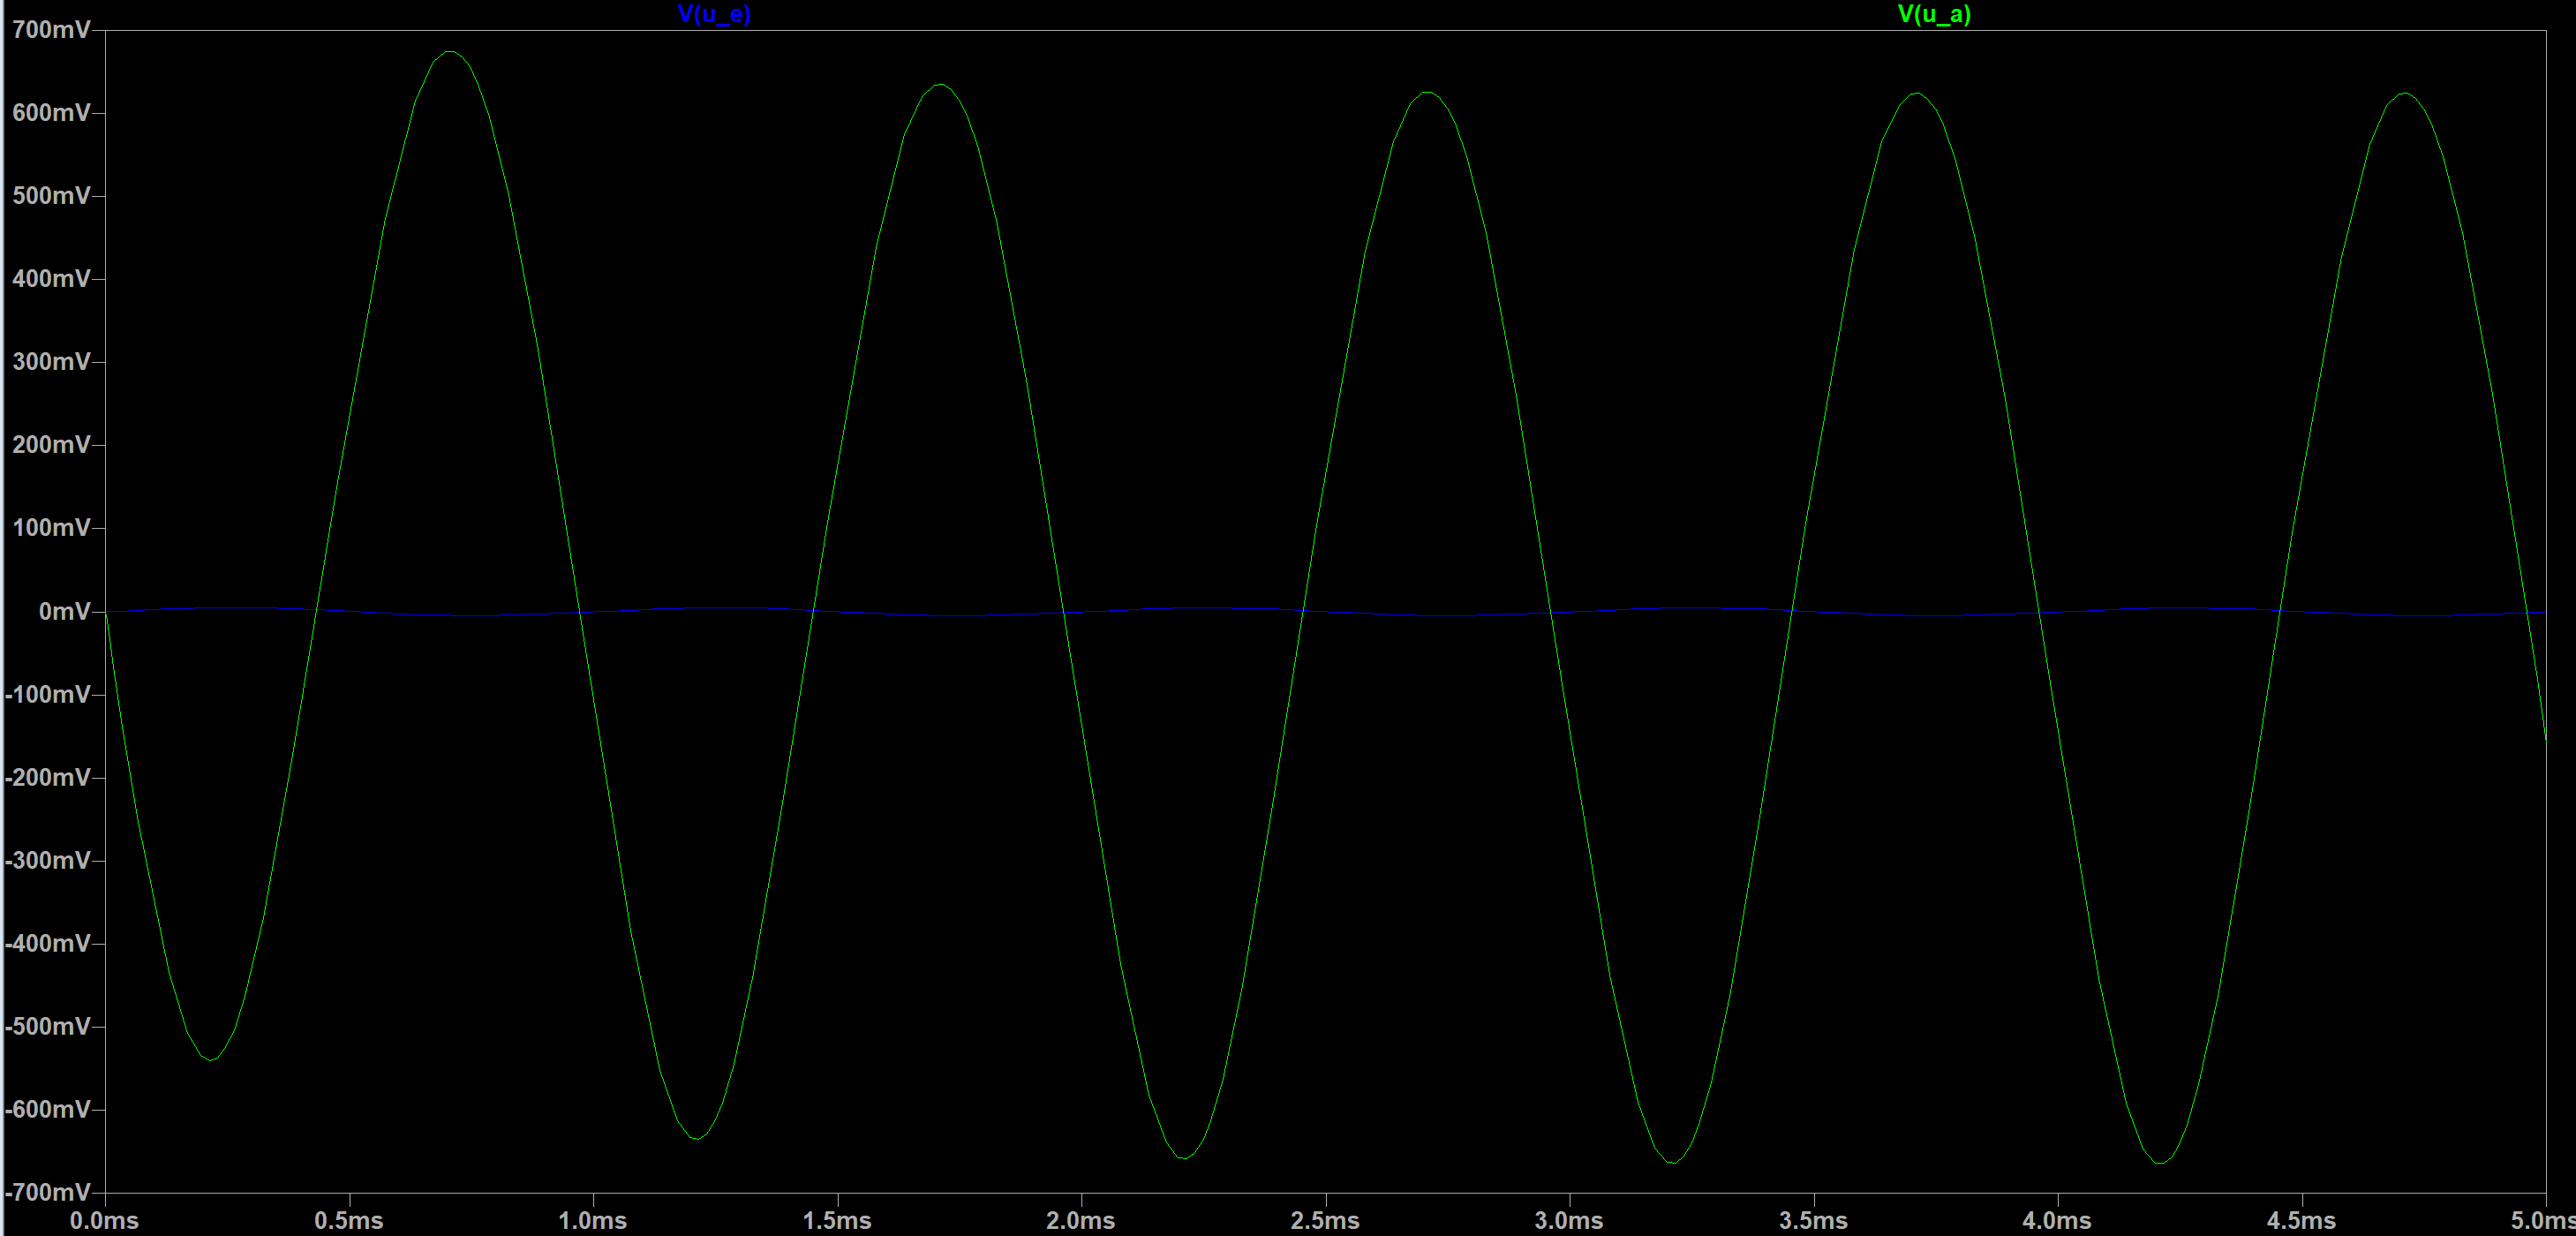
\includegraphics[width=\linewidth, height=7cm]{./figures/mitkond/ausgangssignalmitueberbrueckung.png}
    \caption{Zeitlicher Verlauf der Ausgangsspannung $V(u_a)$
    der Emitterschaltung mit Überbrückungskondensator bei einer Amplitude von
  \SI{5}{mV} des Eingangssignals}
    \label{fig:sim_mit_normal_ausgang}
\end{figure}

% FIXME(MAX) 2.3 Testen Sie wie hoch die maximale Eingangspannung werden darf bis der Transistor in der Simulation
% FIXME(MAX) übersteuert. Übersteuern Sie ihn anschließend und nehmen Sie wieder die Eingangspannung sowie
% FIXME(MAX) die Ausgangsspannung nach der Zeit auf 
% und diskutieren Sie anhand dieses Plots die auftretenden
% Verzerrungen.

\paragraph{Übersteuerungsbetrieb}

% TODO erstellen eines Parametersweep um die Übersteuerungsgrenze gut darzustellen
Um die Übersteuerungsgrenze zu finden. wurde ein Parameter-Sweep durchgeführt,
wobei die Amplitude der Eingangsspannung variiert wurde. Dadurch konnte die
Übersteuerungsgrenze visuell bestimmt werden.



% FIXME(MAX) 2.4 Erstellen Sie einen DC Sweep in Abhängigkeit der Temperatur und zeigen Sie die Änderung des
% FIXME(MAX) Kollektorpotentials. 
% Diskutieren Sie die Konsequenzen einer Temperaturerhöhung.
\paragraph{DC Temperatur Sweep}
%TODO der text
Zur Darstellung der Temperaturabhängigkeit wurde ein DC-Sweep durchgeführt. In \autoref{fig:sim_dc_temp_sweep_mit} ist das Kollektorpotential in Abhängigkeit der Temperatur zu sehen.
% TODO verbessere mich
\begin{figure}[H]
  \centering
    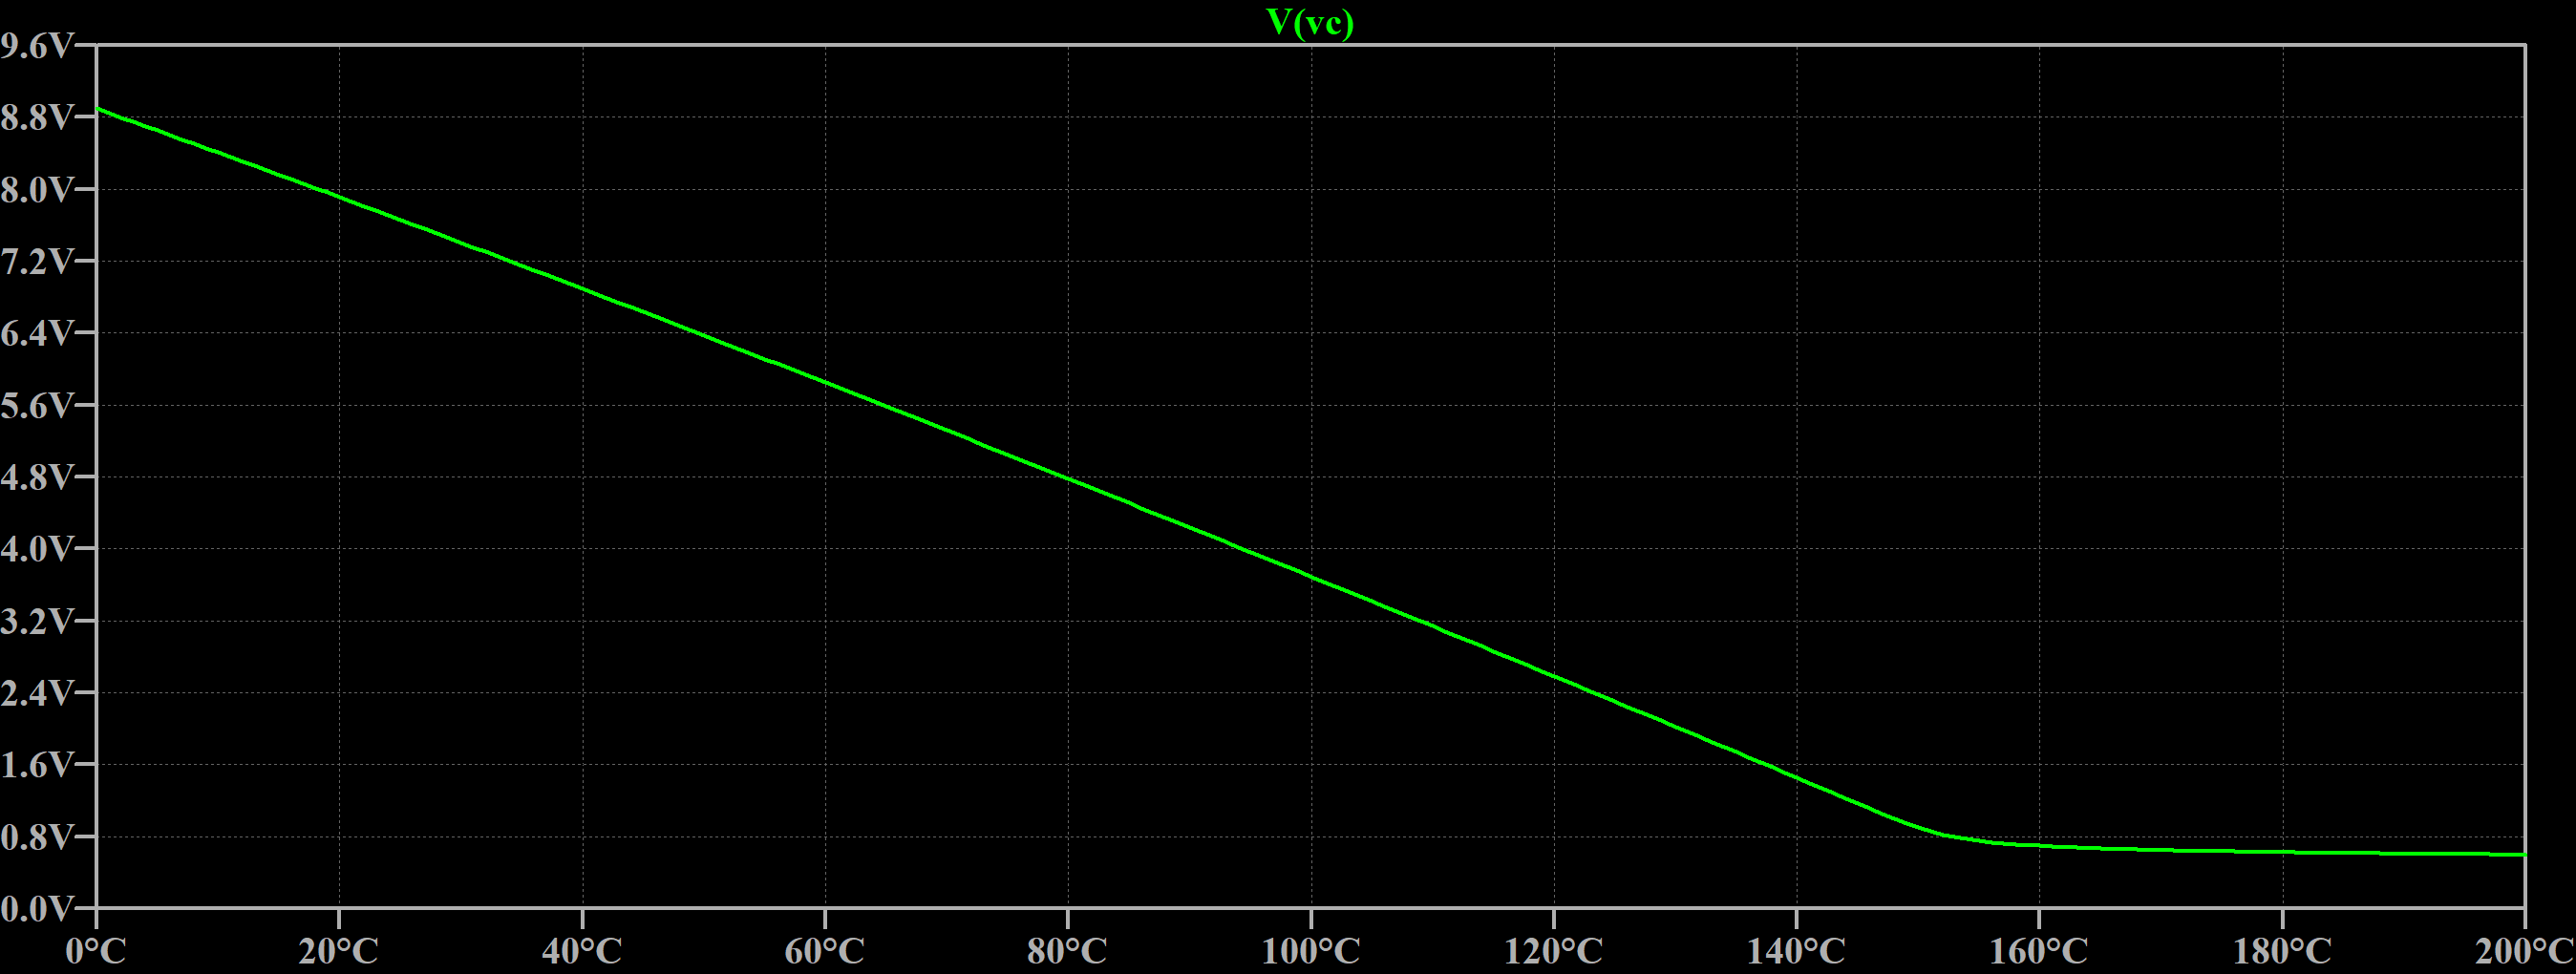
\includegraphics[width=\linewidth, height=7cm]{./figures/mitkond/tempmitkondkollektorpot.png}
    % TODO verbessere mich und ueberpruefe spice directive
    \caption[Simulierter DC Temperatur Sweep mit
    Überbrückungskondensator]{Simulierter DC Temperatur Sweep welcher die
      Temperaturabhängigkeit des Kollektorpotentials darstellt. Auf der
      Abszisse befindet sich die Temperatur des Transistors und auf Ordinate
      befindet sich das Kollektorpotential $VC$. Diese Simulation wurde bei dem
      Schaltplan aus \autoref{fig:schaltungmitkond} mit folgender SPICE
      directive \texttt{.dc temp 0 200 1} durchgeführt.
  }
  \label{fig:sim_dc_temp_sweep_mit}
\end{figure}

% 2.5 Nehmen Sie die Ausgangsspannung über der Zeit für verschiedene Temperaturen in einem
% Diagramm dar und diskutieren Sie diesen Plot.
\paragraph{Temperaturvariierte Transiente Analyse}
%TODO der text
Für die Ausgangsspannung wurde eine temparaturvariierte, transiente Analyse durchgeführt. Für fünf verschiedene Betriebstemperaturen ist der Verlauf der Ausgangsspannung in \autoref{fig:sim_tran_temp_mit} zu sehen.
\begin{figure}[H]
  \centering
    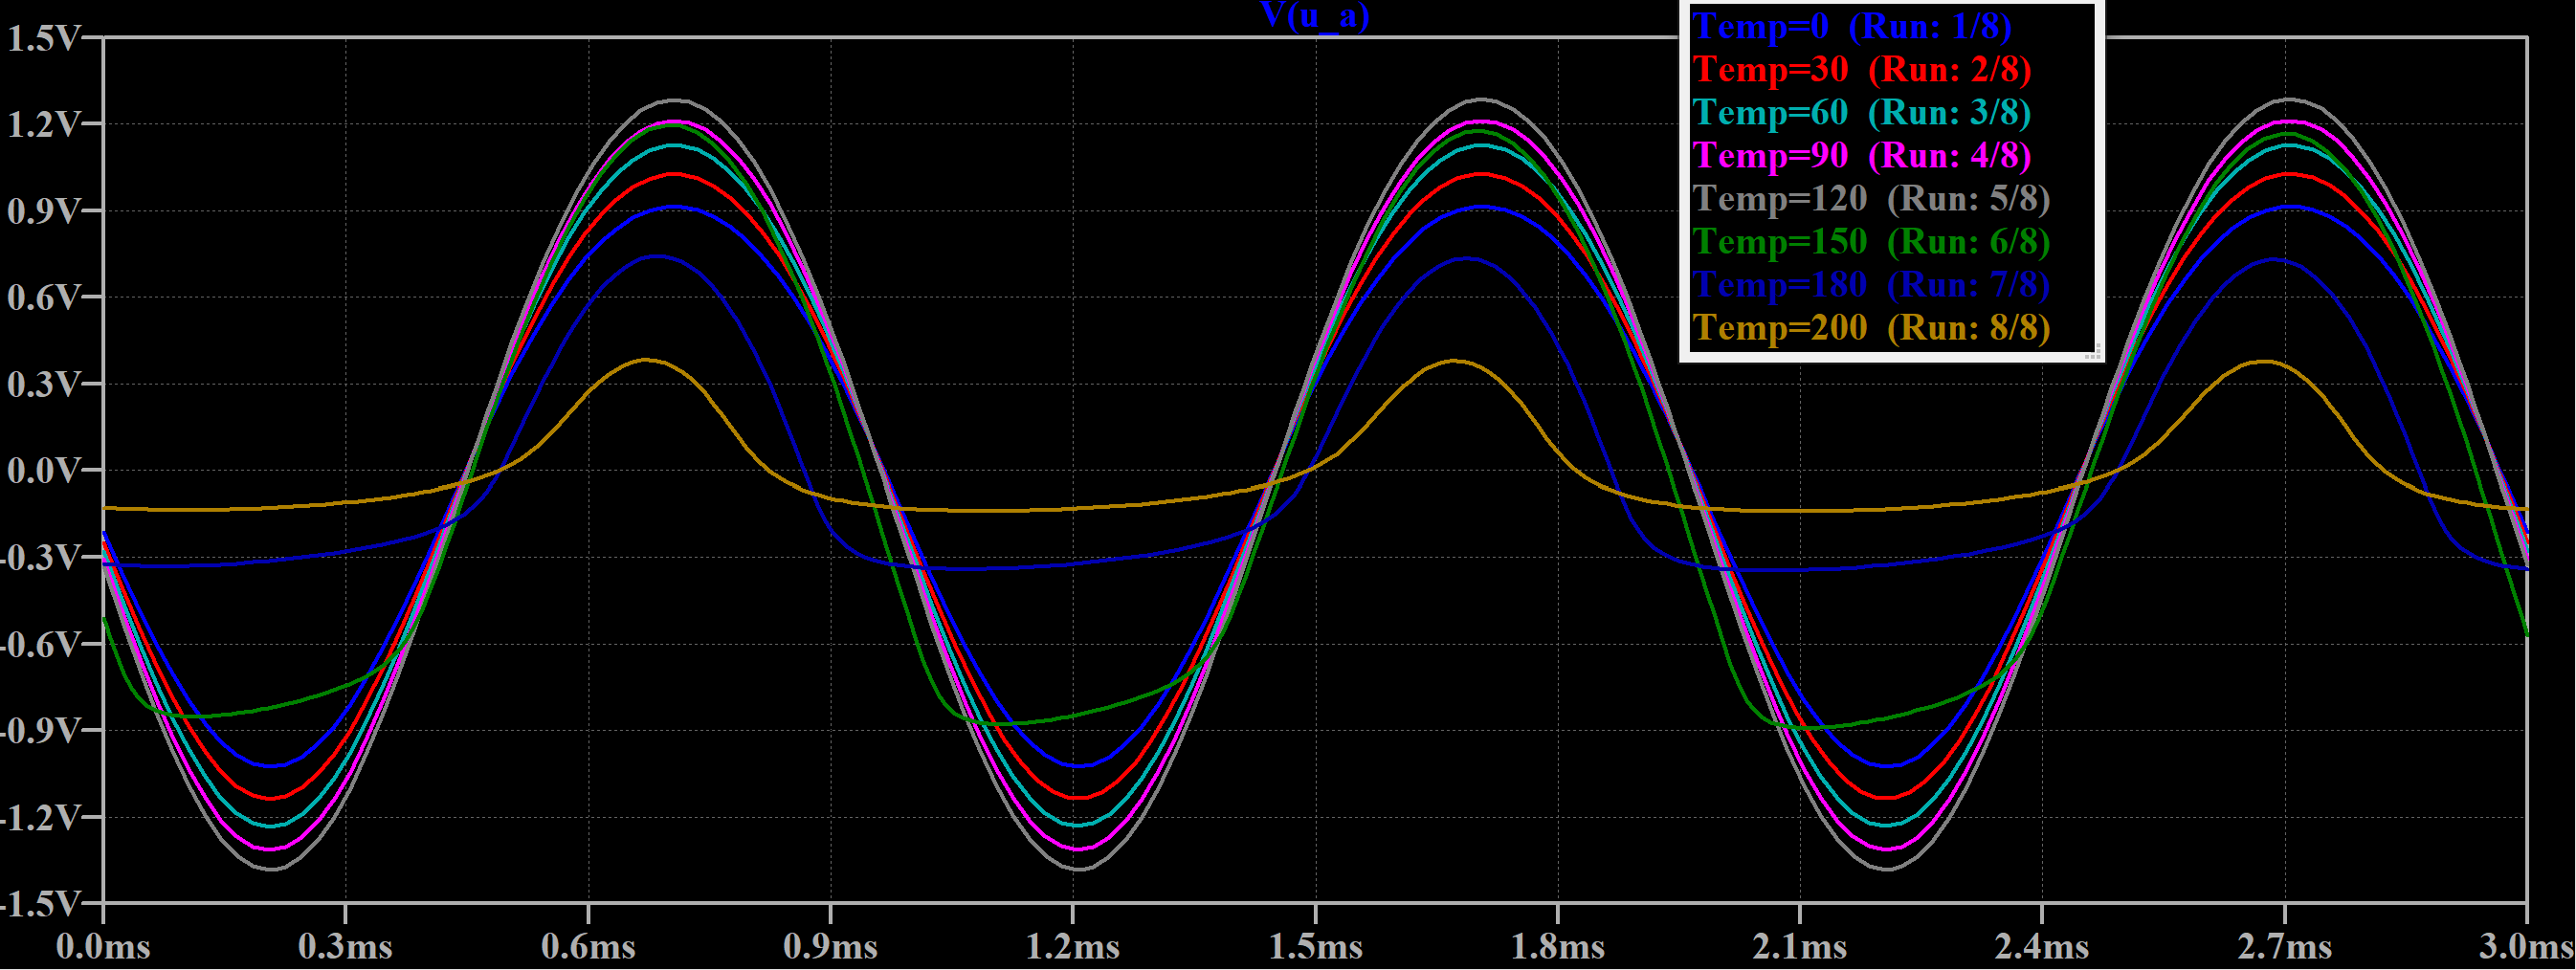
\includegraphics[width=\linewidth, height=7cm]{./figures/mitkond/ausgangmitkondtempsweep20mv.png }
    % TODO verbessere mich und ueberpruefe spice directive
    \caption[Simulierte Transient Analyse mit
    Überbrückungskondensator]{Simulierte Transient Analyse von der
      Ausgangsspannung unter Einfluß verschiedener Betriebstemperaturen. Auf
      der Abszisse befindet sich die Zeit und auf Ordinate befindet sich die
      Ausgangsspannung $U_a$. Diese Simulation wurde bei dem Schaltplan aus
    \autoref{fig:schaltungmitkond} mit folgenden SPICE directives \texttt{.tran
      0 0.005 0 0.0001} und \texttt{.step temp 0 200 50} durchgeführt. Die Legende
    beinhaltet die Zuordnung von Farbe zu Temperatur (in Celsius).}
  \label{fig:sim_tran_temp_mit}
\end{figure}



% 3.1 Auch wenn die Schaltung prinzipiell nicht dafür ausgerichtet ist − bauen Sie RE und CE aus und
% untersuchen Sie die Verstärkung und die Temperaturabhängigkeit des Kollektorpotentials ohne
% jegliche Rückkopplung. (Beachten Sie, dass der Arbeitspunkt dabei unvorteilhaft verschoben wird.)
\subsubsection{Schaltung ohne Emitterwiderstand \& Überbrückungskondensator}
Am Ende wird die Emitterschaltung exklusive dem Emitterwiderstand und wiederum
ohne den Überbrückungskondensator verwendet, um die starke
Temperaturabhängigkeit einer Transistorschaltung darzustellen. Die Schaltung
ist  \autoref{fig:schatlungohnekundre} zu entnehmen.

%TODO: schaltung ohne kond und ohne re foto machen
\begin{figure}[H]
    \centering
    % 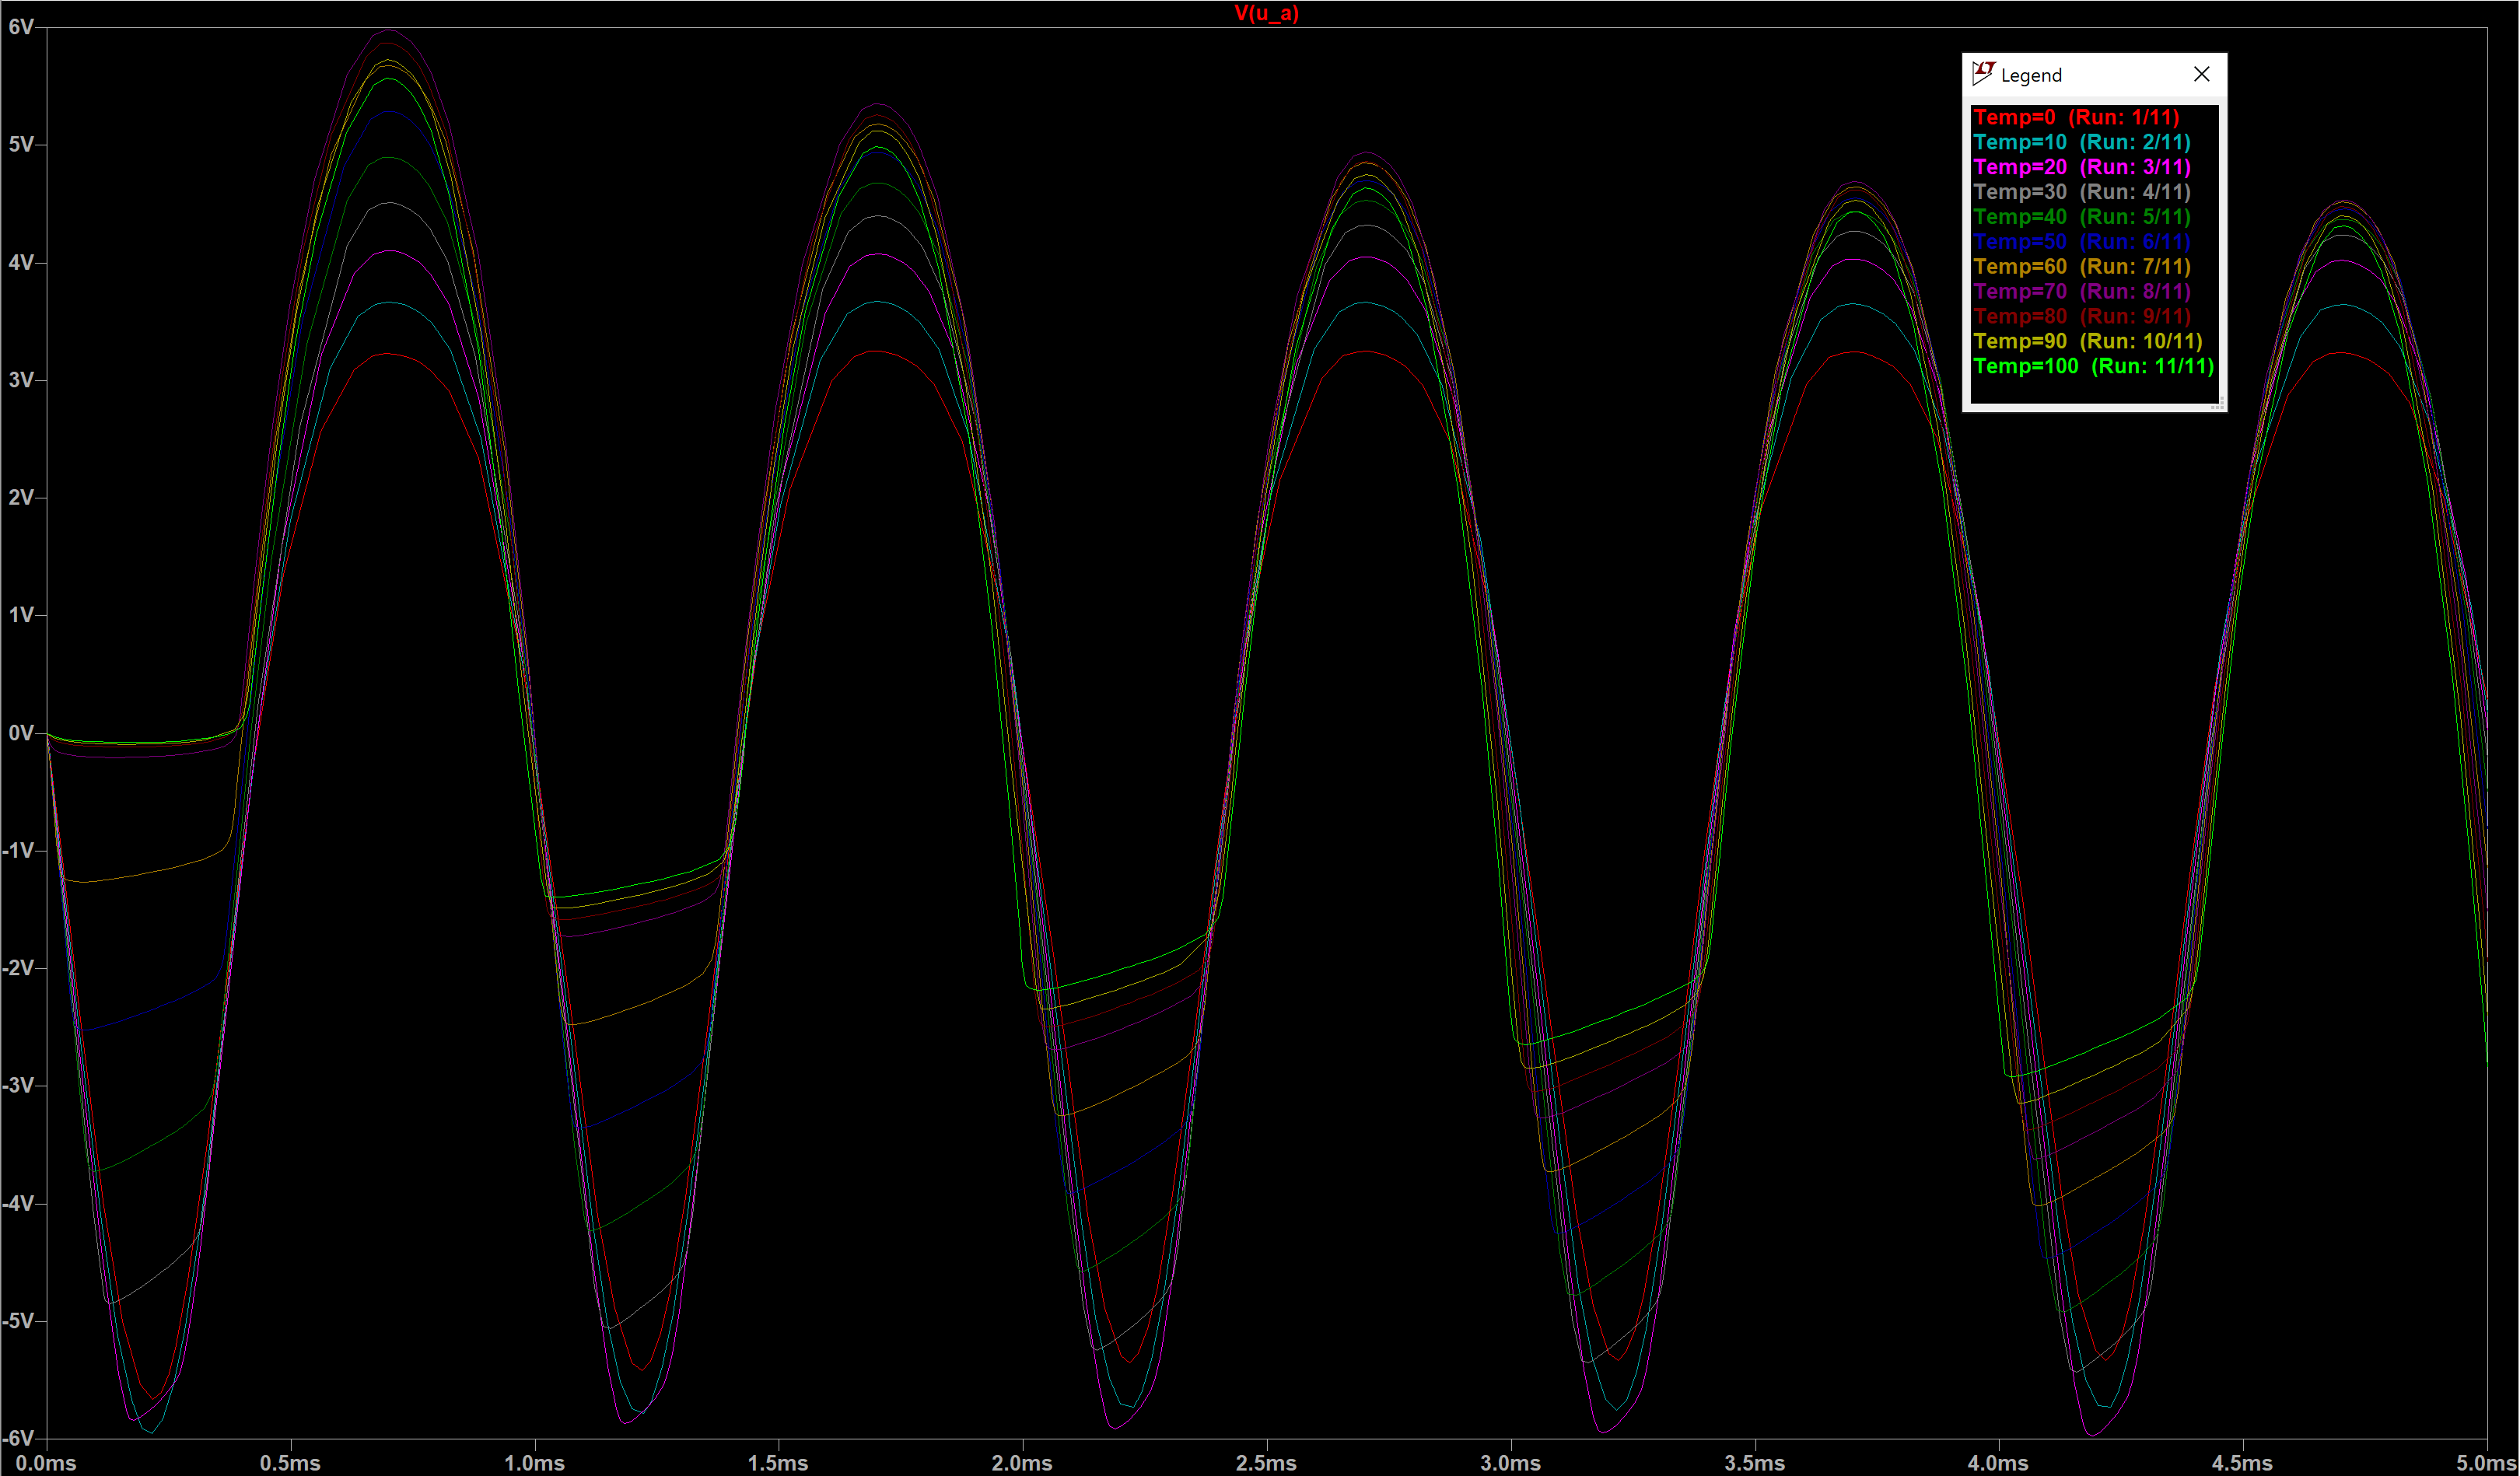
\includegraphics[width=8cm, height=8cm,keepaspectratio]{./figures/ohnekondundre/temperaturausgang50mvr2auf10kohm.png}
    \caption{Schaltung mit Überbrückungskondensator bei einem Sinus-Eingangssignal
      mit einer Amplitude von \SI{6}{\milli\volt}, einer Frequenz von \SI{1}{\kilo\hertz} und einem
      Innenwiderstand von \SI{600}{\ohm} ; mit der Eingangs- $U_e$ und
      Ausgangsspannung $U_a$, den Eingangs- $Ce$ und Ausgangskondensatoren $Ca$, den
      Vorwiderständen $R1$ und $R2$, dem Kollektorwiderstand $RC$, dem
      Emitterwiderstand $RE$, dem Lastwiderstand $RL$, dem Basispotential $Vb$, dem
      Kollektorpotential $Vc$, dem Transistor \textit{BC107B} und der
      Betriebsspannung $UB$. Genauere Spezifikationen können dem Schaltbild entnommen
      werden.}
    \label{fig:schatlungohnekundre}
\end{figure}

Die Spannungsverläufe für die Schaltung ohne Emitterwiderstand und
Überbrückungskondensator sind in \autoref{fig:verlaufohnekondundre} zu
sehen.
\begin{figure}
  \centering
  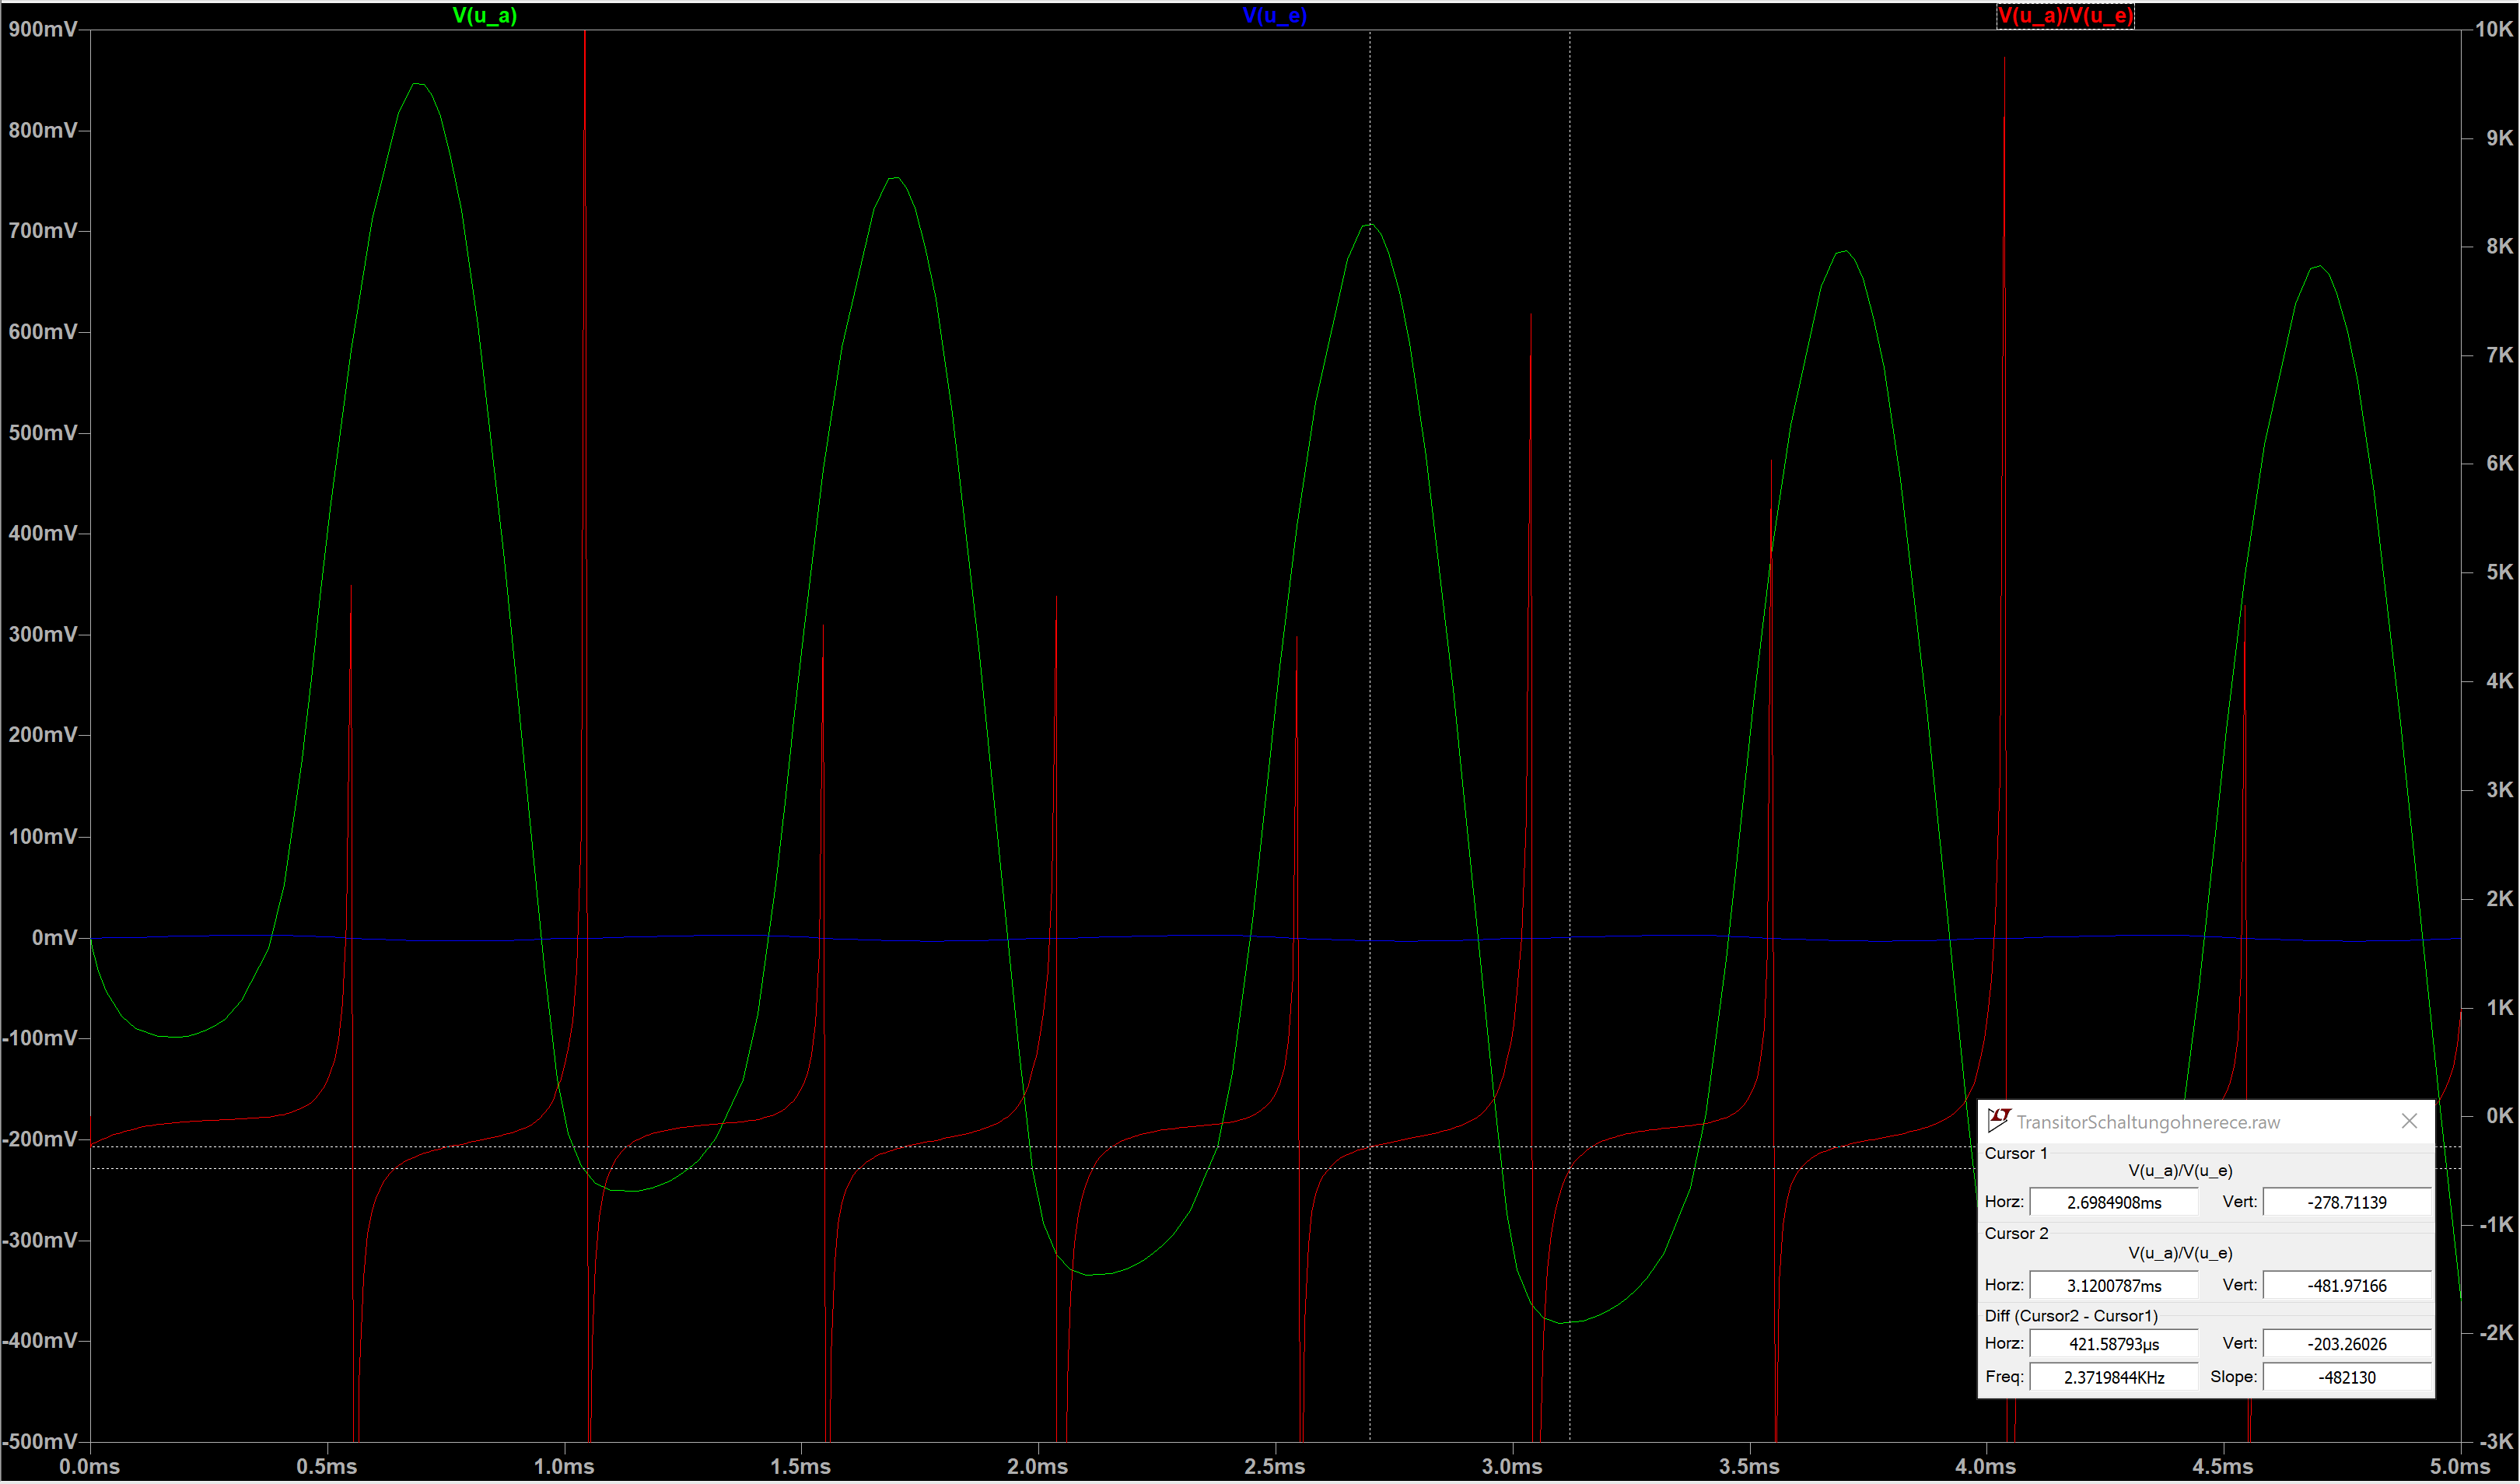
\includegraphics[width=\linewidth, height=7cm]{./figures/ohnekondundre/verstaerkung5mv.png}
% TODO verbessern 
  \caption{Spannungsverläufe für die Schaltung ohne $RE$ und $CE$}
  \label{fig:verlaufohnekondundre}
\end{figure}

\paragraph{DC Temperatur Sweep}
Zur Darstellung der Temperaturabhängigkeit wurde ein DC-Sweep durchgeführt. In \autoref{fig:sim_dc_temp_sweep_ohne_ohne_re} ist das Kollektorpotential in Abhängigkeit der Temperatur zu sehen.
\begin{figure}[H]
  \centering
    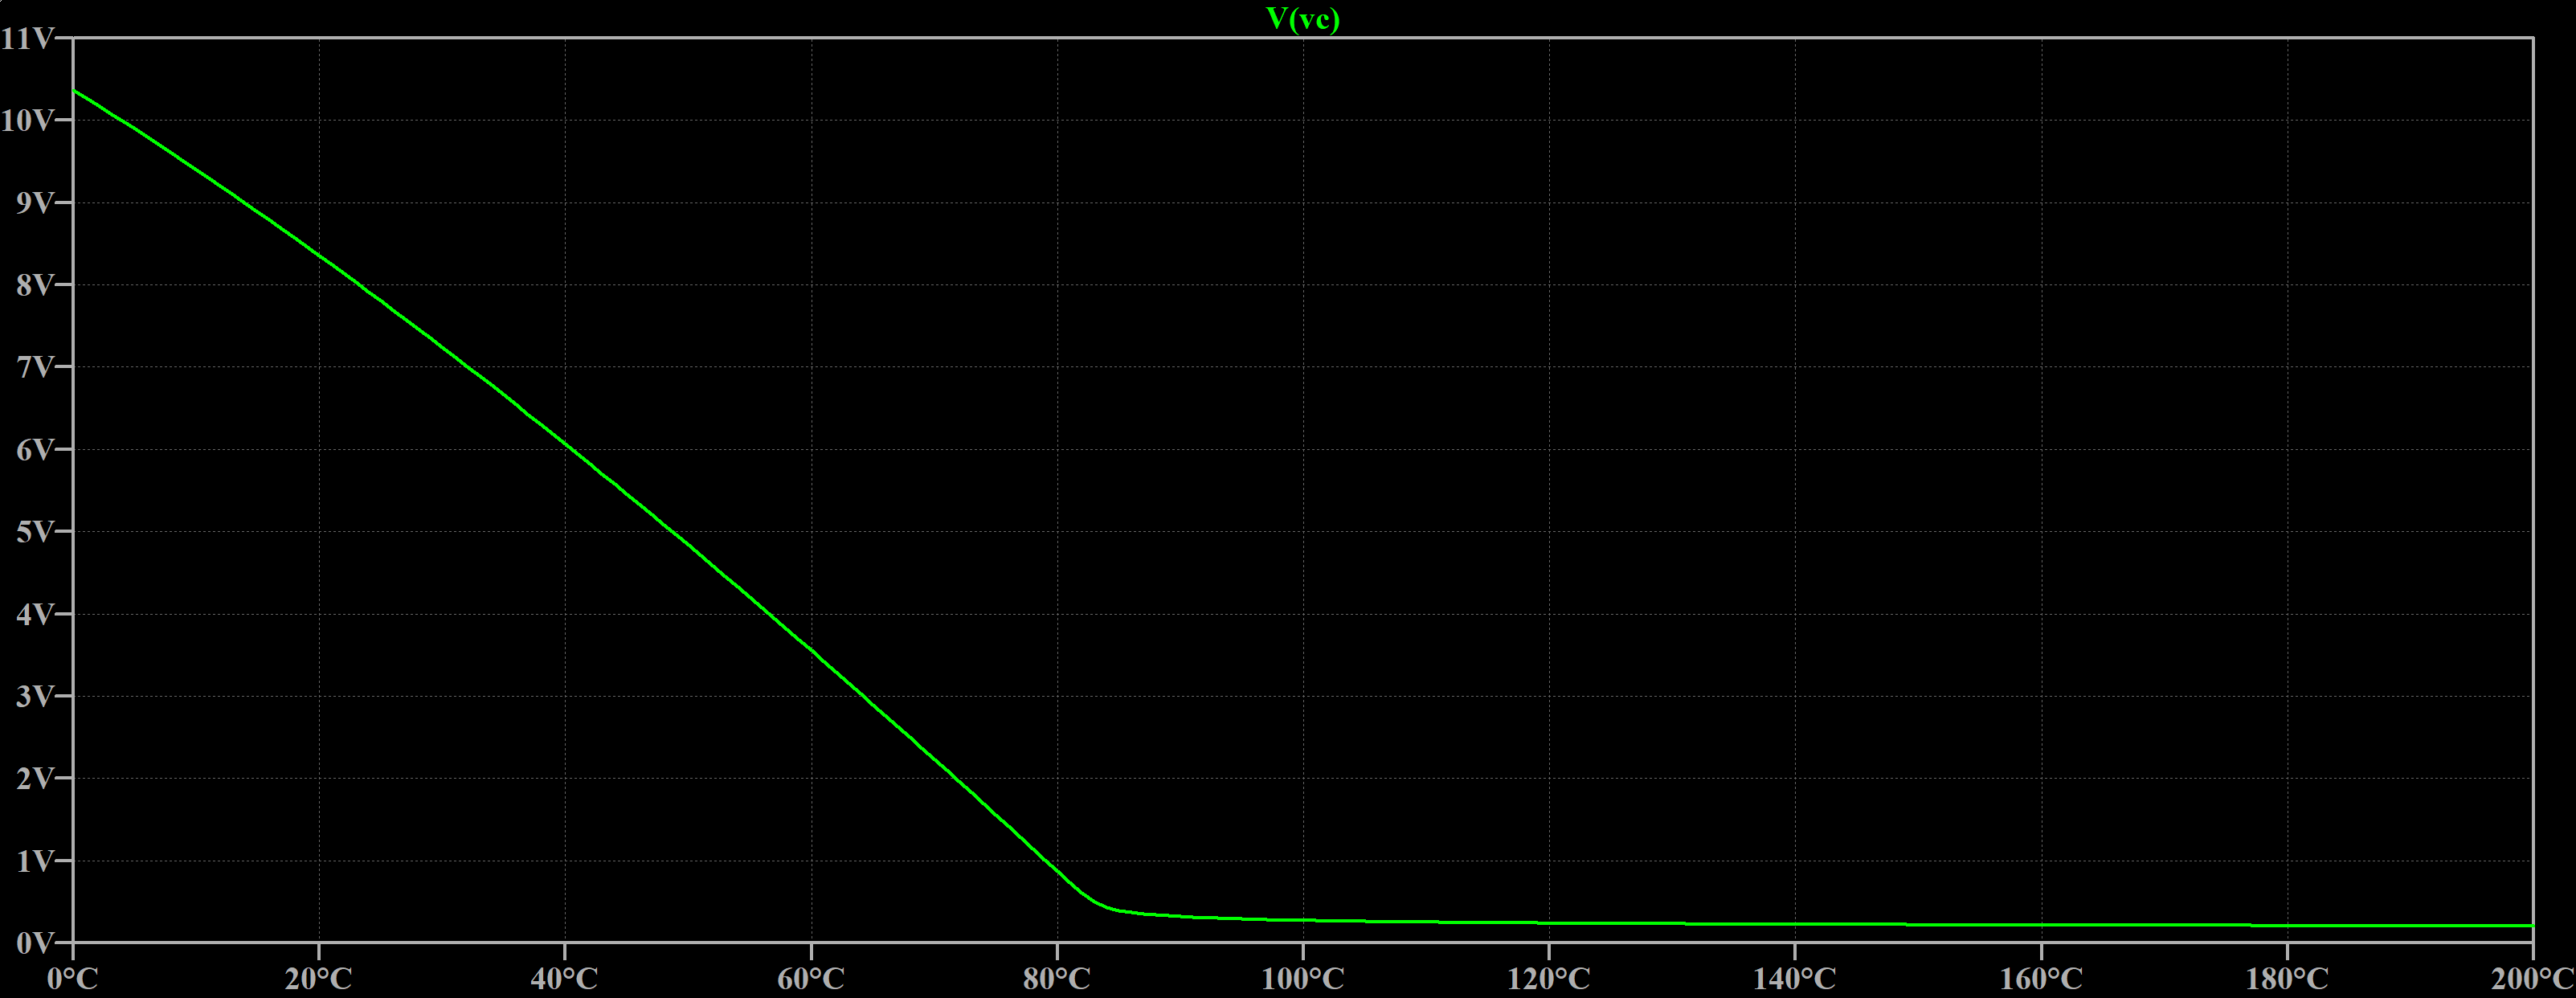
\includegraphics[width=\linewidth, height=7cm]{./figures/ohnekondundre/dcsweepkollektorpotR2auf10kohm5mv.png }
    % TODO verbessere mich und ueberpruefe spice directive
    \caption[Simulierter DC Temperatur Sweep ohne
    Überbrückungskondensator und ohne Emitterwiderstand]{Simulierter DC Temperatur Sweep welcher die
      Temperaturabhängigkeit des Kollektorpotentials darstellt. Auf der
      Abszisse befindet sich die Temperatur des Transistors und auf Ordinate
      befindet sich das Kollektorpotential $VC$. Diese Simulation wurde bei dem
      Schaltplan aus \autoref{fig:schatlungohnekundre} mit folgender SPICE
      directive \texttt{.dc temp 0 200 1} durchgeführt.
  }
  \label{fig:sim_dc_temp_sweep_ohne_ohne_re}
\end{figure}

\paragraph{Temperaturvariierte Transiente Analyse}
%TODO der text
Für die Ausgangsspannung wurde eine temparaturvariierte, transiente Analyse durchgeführt. Für elf verschiedene Betriebstemperaturen ist der Verlauf der Ausgangsspannung in \autoref{fig:sim_tran_temp_ohne} zu sehen.
\begin{figure}[H]
  \centering
    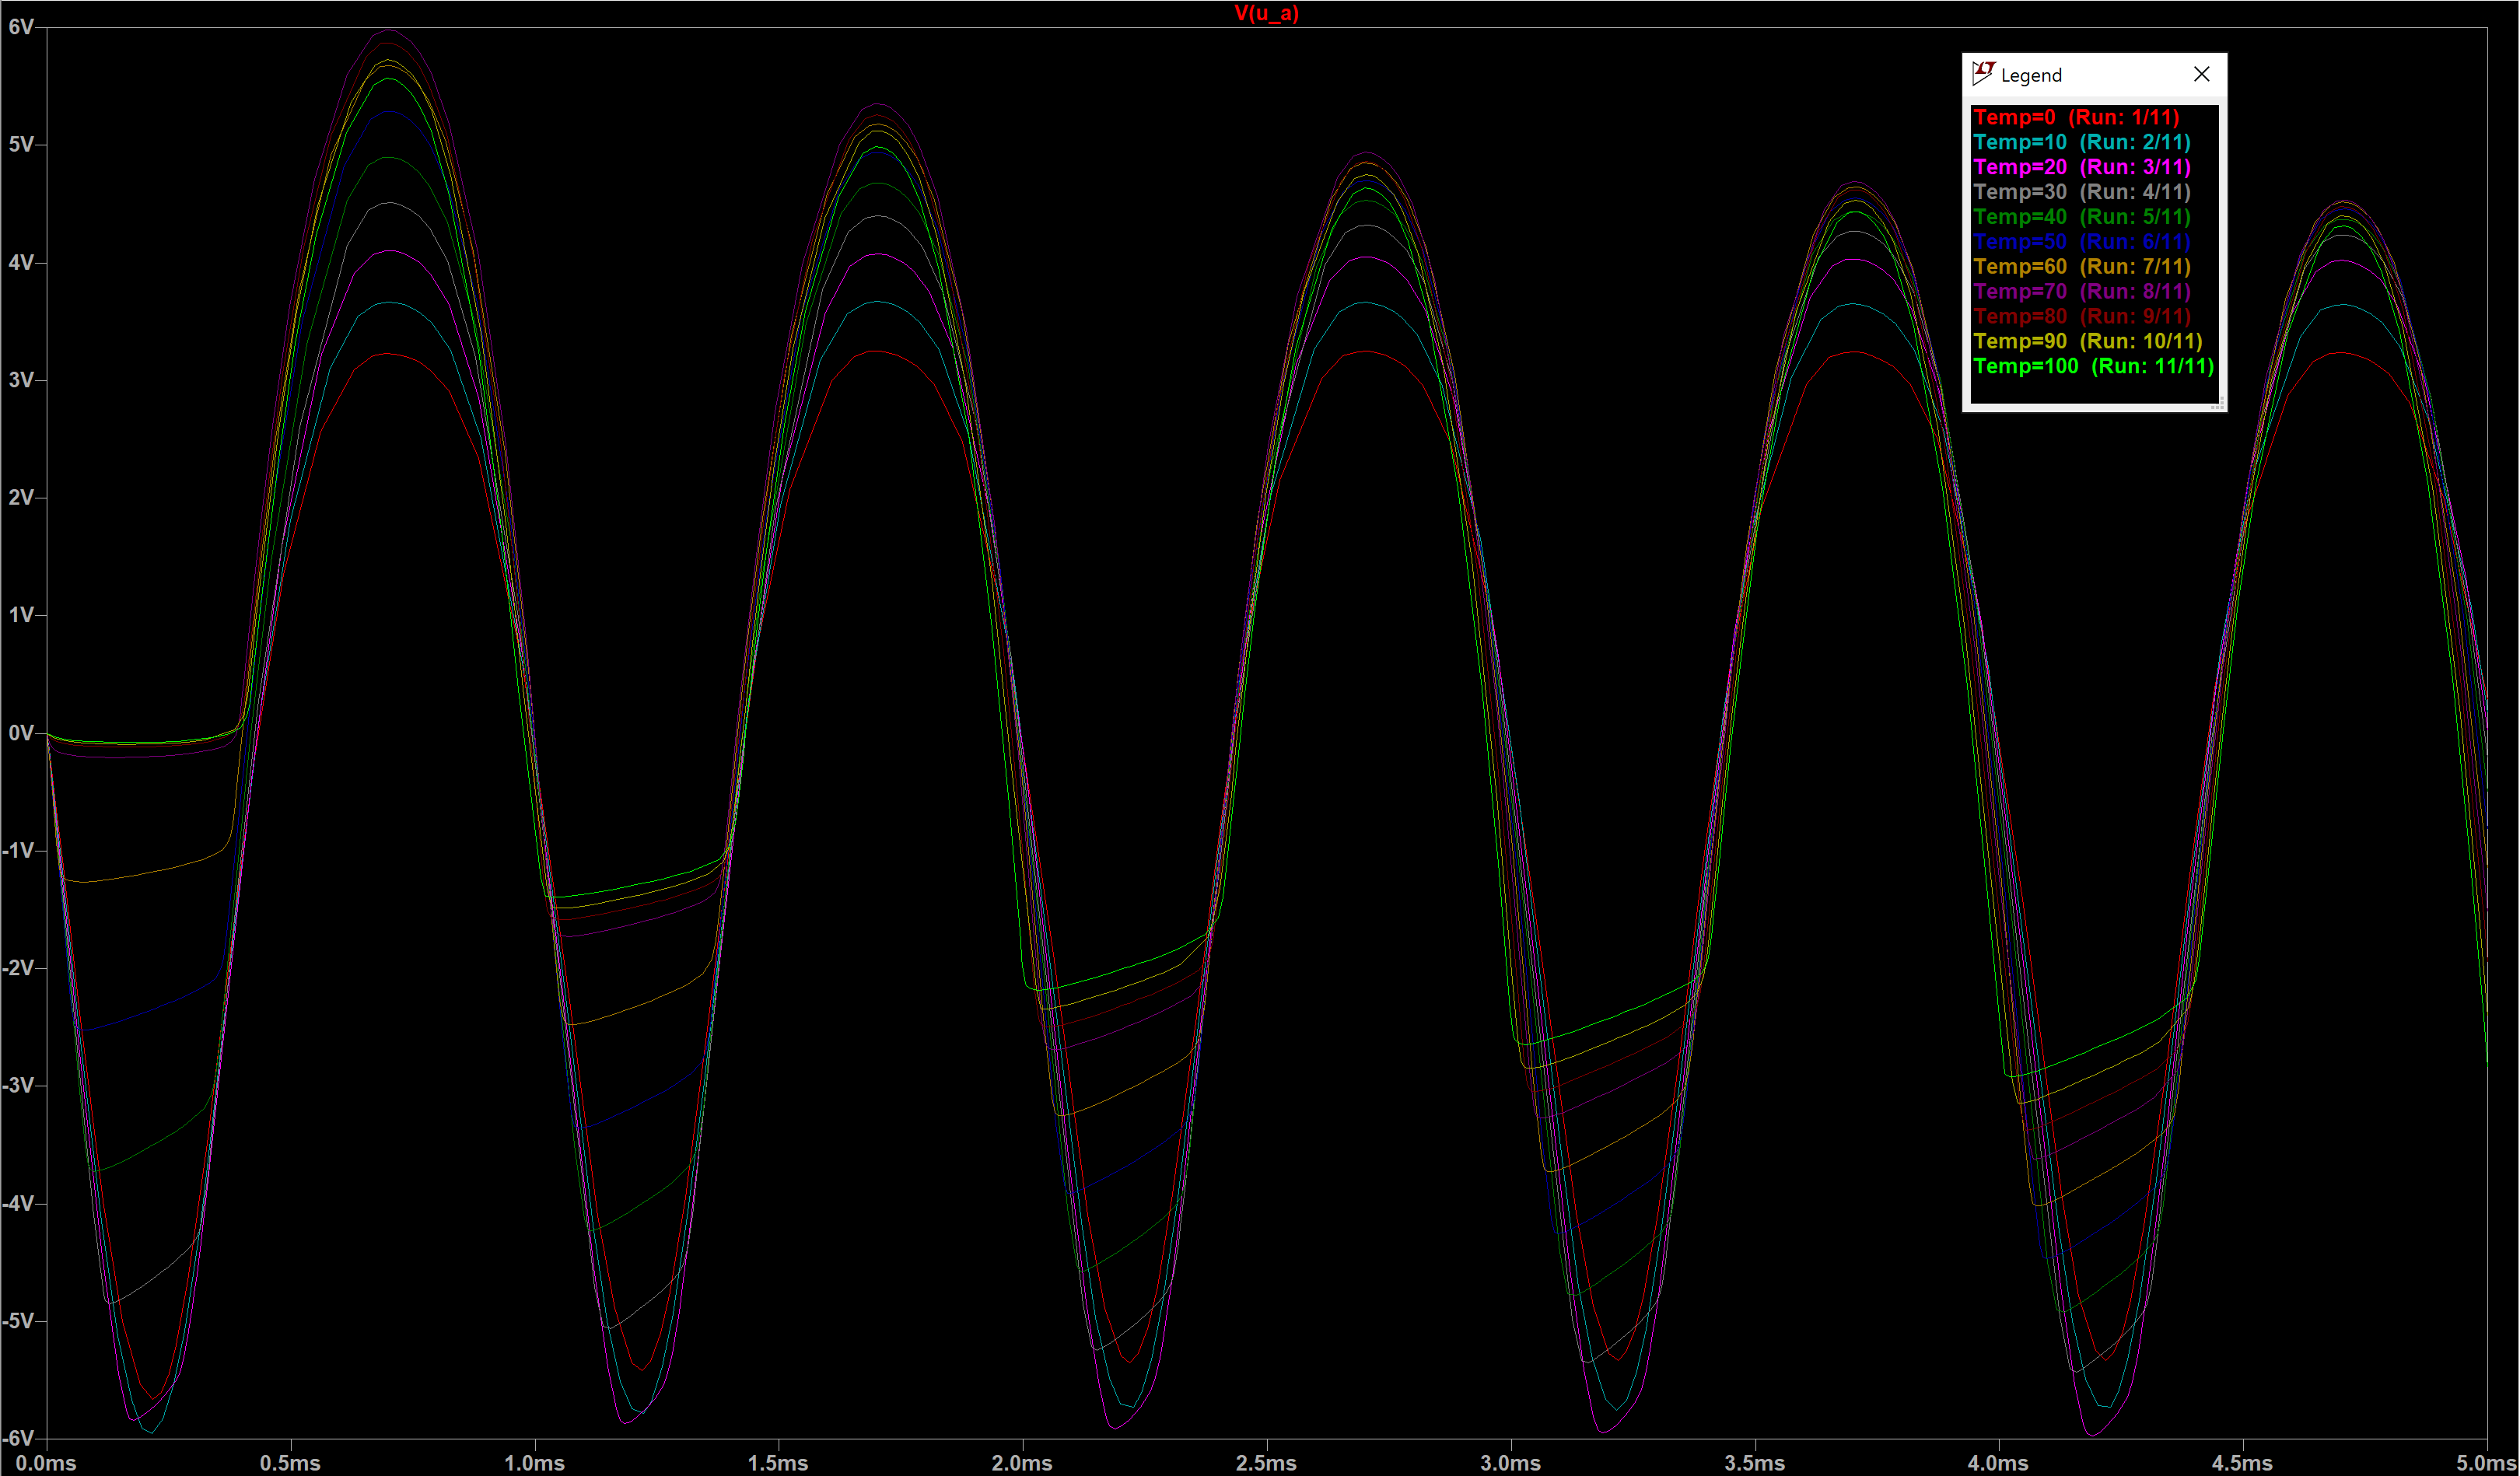
\includegraphics[width=\linewidth, height=7cm]{./figures/ohnekondundre/temperaturausgang50mvr2auf10kohm.png }
    % TODO verbessere mich und ueberpruefe spice directive
    \caption[Simulierte Transient Analyse mit
    Überbrückungskondensator]{Simulierte Transient Analyse von der
      Ausgangsspannung unter Einfluß verschiedener Betriebstemperaturen. Auf
      der Abszisse befindet sich die Zeit und auf Ordinate befindet sich die
      Ausgangsspannung $U_a$. Diese Simulation wurde bei dem Schaltplan aus
    \autoref{fig:schatlungohnekundre} mit folgenden SPICE directives \texttt{.tran
      0 0.005 0 0.0001} und \texttt{.step temp 0 100 10} durchgeführt. Die Legende
    beinhaltet die Zuordnung von Farbe zu Temperatur (in Celsius).}
  \label{fig:sim_tran_temp_ohne_ohne_re}
\end{figure}

% 1.1 Bauen Sie die Schaltung am Steckboard gemäß der berechneten Parameter ohne den Kondensator CE
% auf. Nähern Sie sich bei Ihren berechneten Widerstandswerten durch Serienschaltung der
% vorhandenen Fixwiderstände der Reihe E12 auf ein vernünftiges Maß an. Führen sie den
% Eingangsspannungsteiler mit einem Fixwiderstand und einem Potentiometer aus um den
% Arbeitspunkt anpassen zu können. Notieren Sie die tatsächlich verwendeten Widerstandswerte
% (messen Sie hierfür die Widerstände aus, diese weichen nämlich teilweise erheblich von ihrem
% nominellen Wert ab).
\subsection{Steckbrett}
Für den praktischen Teil an der Steckplatine werden Widerstände der E12-Reihe
verwendet. Zusätzlich wird für die Vorwiderstände im Spannungsteiler ein
seriell geschaltetes Potentiometer verwendet, mit welchem man sich an den
berechneten Arbeitspunkt für die Emitterschaltung annähert. 

%todo:geraeteliste
Die verwendeten Geräte sind \autoref{tab:geraeteliste} zu entnehmen.

\begin{table}
  \caption{Tabelle der verwendeten Geräte}
  \label{tab:geraeteliste}
  \centering
  \begin{tabular}{l|l}
    \hline
   \multicolumn{2}{ c }{\textbf{Geräteliste}} \\
    \hline
    \textbf{Gerät} & \textbf{Typ} \\
    \hline
    Oszilloskop & \textit{Tektronix TDS 2002}\\
    Funktionsgenerator & \textit{FG250D} \\
    Netzgerät & nicht bestimmbar\\
    Multimeter & \textit{Fluke 175 TrueRMS}\\
    Widerstände & siehe \autoref{tab:messung_widerstaende} \\
    Kondensator $C_e$ & \SI{330(40)}{\nano\farad} \\
    Kondensator $C_a$ & \SI{680(70)}{\nano\farad}\\
    Kondensator $C_E$ & \SI{270(30)}{\micro\farad}\\
    \hline
  \end{tabular}
\end{table}

\begin{table}[H]
  \caption{Gemessene Werte der Widerstände im Steckbrett. Diese Messungen sind
  mit dem \textit{Fluke 175 TrueRMS} gemessen worden. \\
  $R_C \dots$  Kollektorwiderstand\\
  $R_E \dots$  Emitterwiderstand\\
  $R_L \dots$  Lastwiderstand\\
  $R_1 \dots$  Erster Spannungsteilerwiderstand\\
  $R_2 \dots$  Zweiter Spannungsteilerwiderstand
  }
  \label{tab:messung_widerstaende}
  \centering
  \begin{tabular}[c]{l|l}
    $R_C$ & \SI{1.796(18)}{\kilo\ohm} \\
    $R_E$ & \SI{47.4(7)}{\ohm} \\
    $R_L$ & \SI{2.20(3)}{\kilo\ohm} \\
    $R_1$ & \SI{176.0(17)}{\kilo\ohm} \\
    $R_2$ & \SI{11.28(12)}{\kilo\ohm}
  \end{tabular}
\end{table}



Nachdem die Schaltung, wie in  \autoref{fig:aufbau} zu sehen, aufgebaut
wurde, wurden die Spannungsverläufe am Ein- und Ausgang mittels einem
Oszilloskop dargestellt und die Oszillagramme für die nachfolgende
Auswertung exportiert.

\begin{figure}[H]
    \centering
    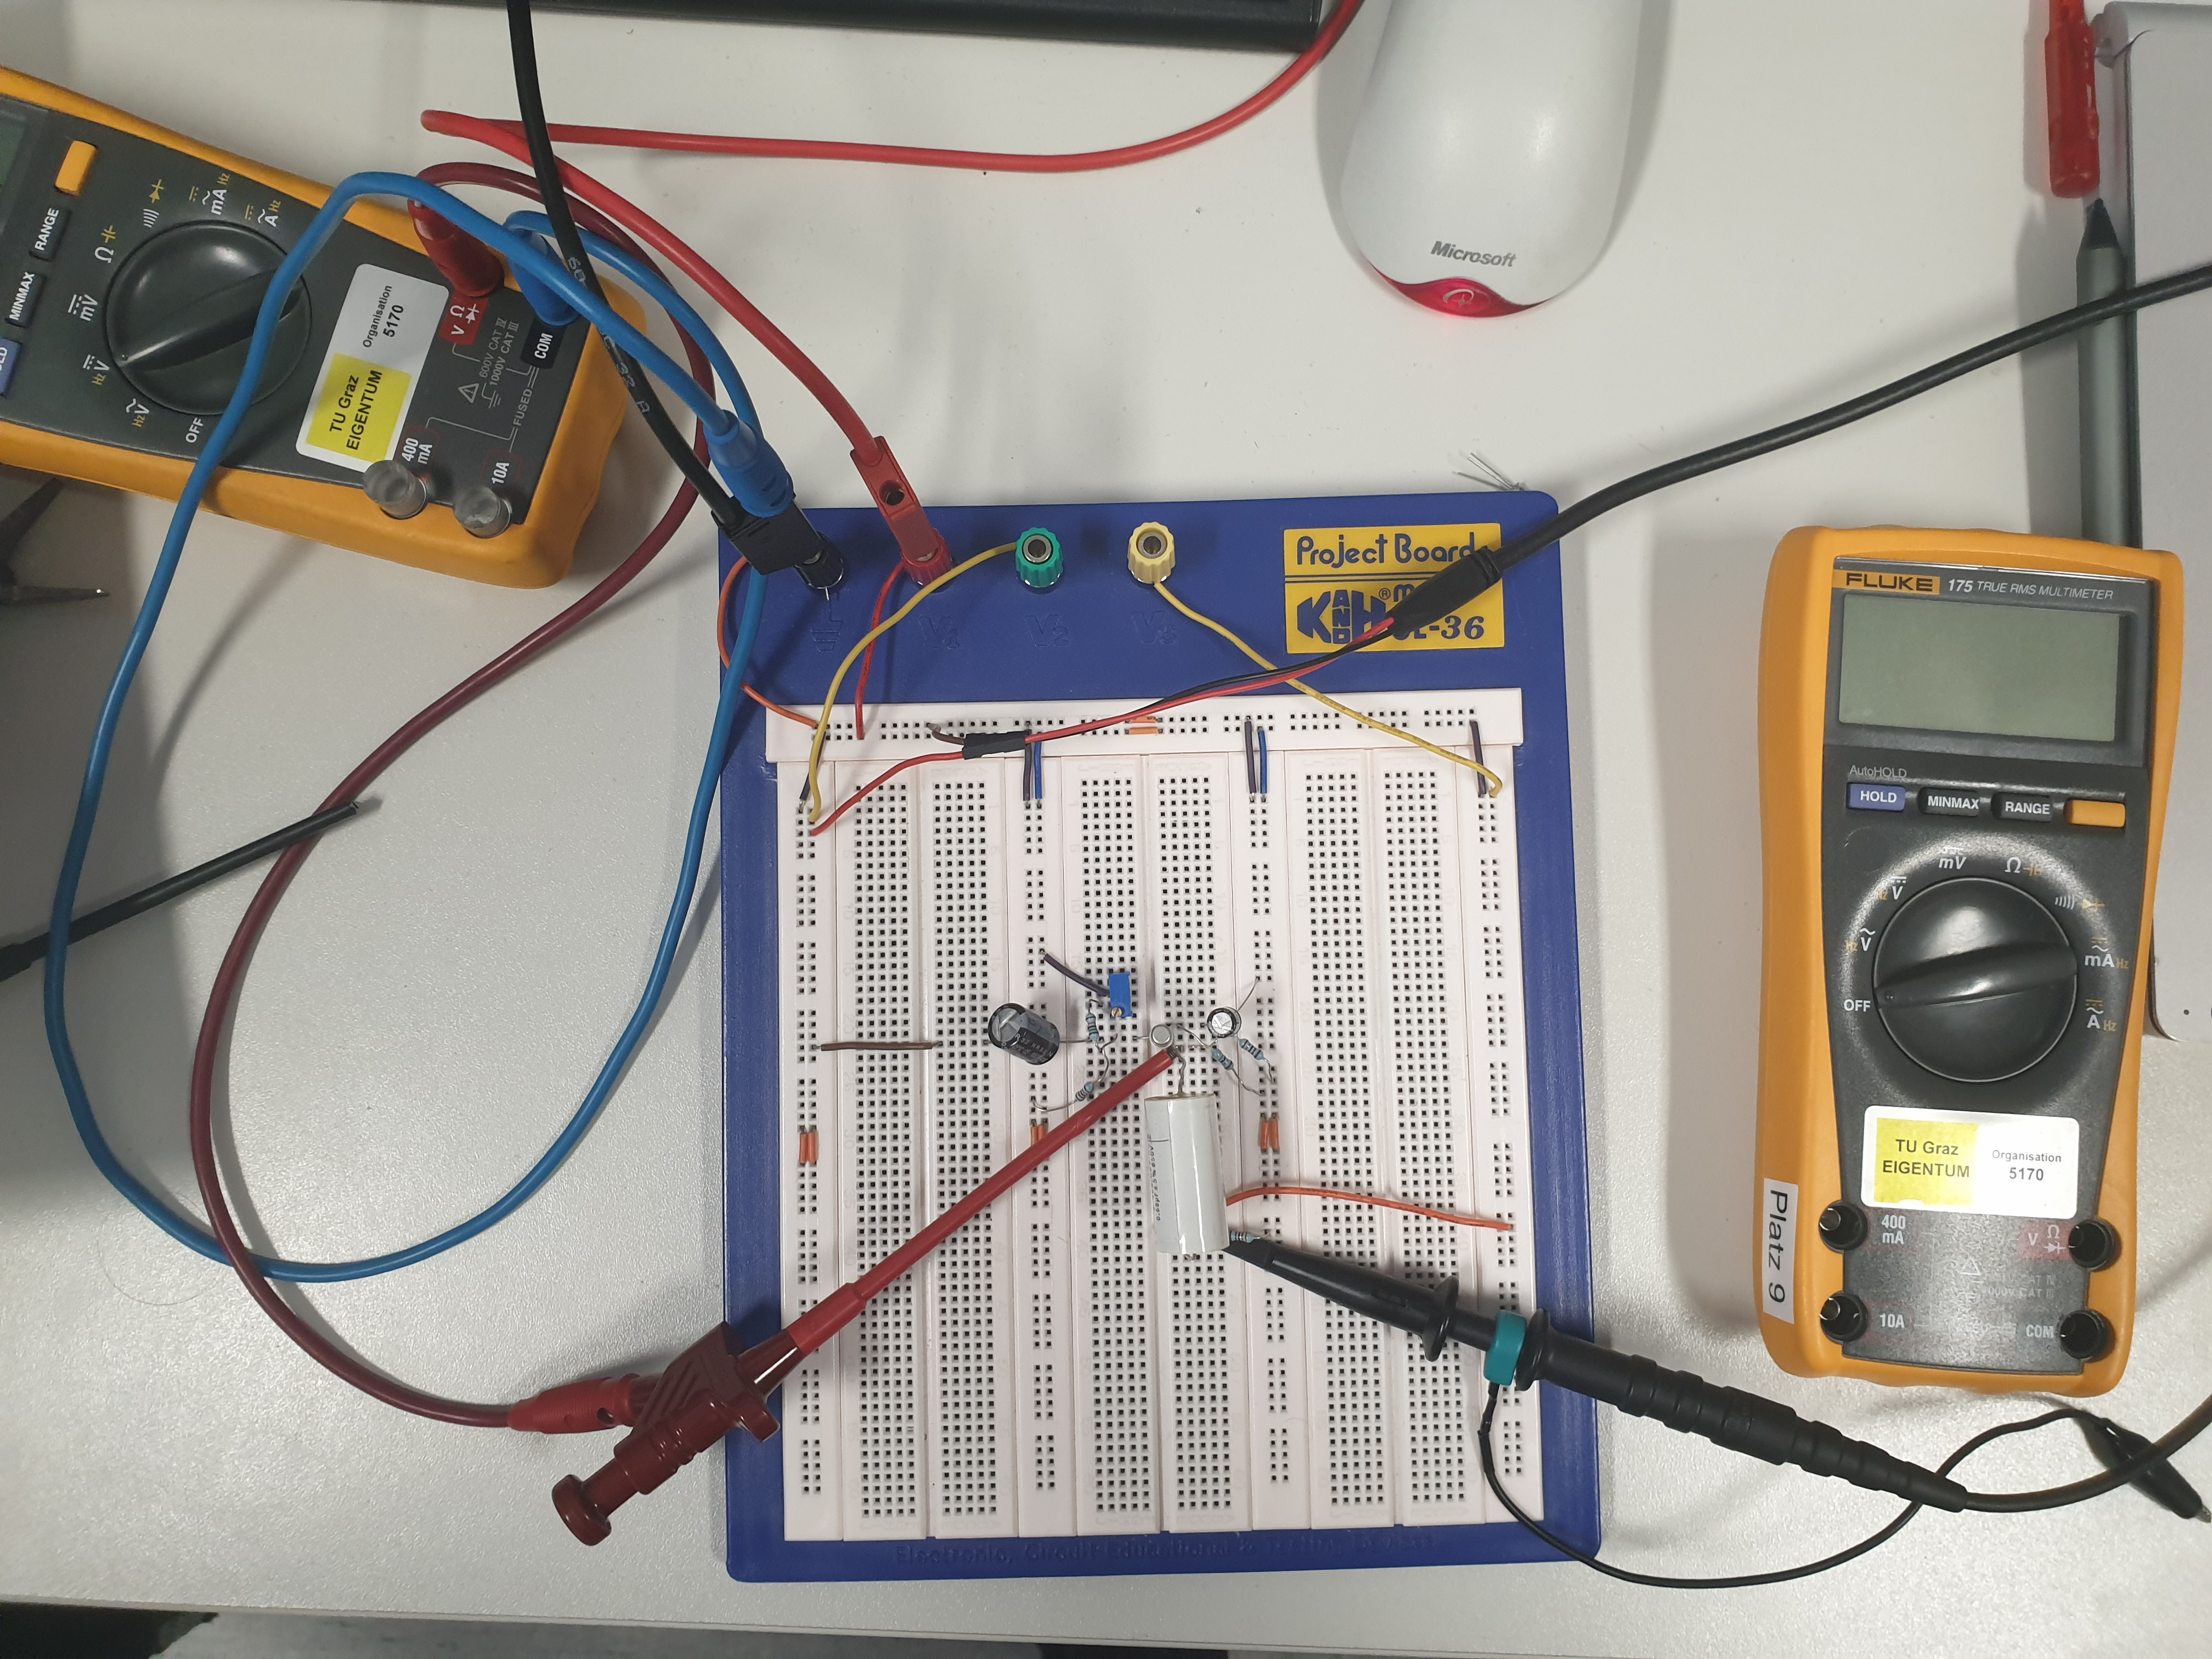
\includegraphics[width=8cm, height=8cm,keepaspectratio]{./figures/foto.png}
    \caption{Am Steckbrett aufgebaute Emitterschaltung mit Überbrückungskondensator}
    \label{fig:aufbau}
\end{figure}



% 1.2 (Überprüfen der Schaltung durch einen Betreuer bevor Inbetriebnahme!)
% Verwenden Sie das Netzgerät für eine konstante Versorgungsspannung messen Sie das
% Kollektorpotential VC,A, stellen Sie es wenn nötig mit Hilfe des Potentiometers auf den gewünschten
% Wert ein. Protokollieren Sie die angepassten Widerstandswerte und die folgenden Größen UCE, UBE,
% VC, VB, IC, IB um den Arbeitspunkt evaluieren zu können.

\begin{table}[H]
  %TODO caption noch verbessern
  \caption{Tabelle mit Messwerten des Arbeitspunkt. Diese Messungen sind
  mit dem \textit{Fluke 175 TrueRMS} gemessen worden. \\
  $U_{CE} \dots$ Kollektoremitterspannung \\
  $U_{BE} \dots$ Basisemitterspannung \\
  $V_C \dots$  Kollektorpotential \\ 
  $V_B \dots$  Basispotential \\ 
  $U_{RC} \dots$ Spannungsabfall über Kollektorwiderstand  \\ 
  $U_{R1} \dots$ Spannungsabfall über $R_1$ \\
  $U_{R2} \dots$ Spannungsabfall über $R_2$
}
  \label{tab:messugenarbeitspunkt}
  \centering
  \begin{tabular}[c]{l|l}
    $U_{CE}$ &  \SI{7.22(18)}{\volt} \\
    $U_{BE}$ &  \SI{645(16)}{\milli\volt} \\
    $V_C$    &  \SI{7.48(18)}{\volt} \\
    $V_B$    &  \SI{900(30)}{\milli\volt} \\
    $U_{RC}$ &  \SI{7.70(19)}{\volt} \\
    $U_{R1}$ &  \SI{14.1(4)}{\volt} \\
    $U_{R2}$ &  \SI{840(20)}{\milli\volt}
  \end{tabular}
\end{table}


% 1.3 (Überprüfen der Schaltung durch einen Betreuer bevor Inbetriebnahme!)
% Stellen Sie nun eine sinusförmige Wechselspannung mit Hilfe des Funktionsgenerators von 1kHz
% ein und benützen Sie dieses Signal als Eingangssignal für Ihre Schaltung. Stellen Sie nun die
% Eingangspannung und die Ausgangsspannung mittels Oszilloskop dar und zwar jeweils mit und
% ohne CE. Laden Sie die Bilder oder wahlweise die Daten mittels dem Programm Open Choice
% Desktop herunter, diskutieren Sie diese, berechnen Sie die Verstärkungen und vergleichen Sie die
% Daten mit der Simulation.

\subsubsection{Normalbetrieb}
%TODO Einfuegen von Bilder mit Messwerten

Die Oszillogramme der Spannungsverläufe sind in \autoref{fig:oszi_ohne_normal}
und \autoref{fig:oszi_mit_normal} dargestellt. 

\paragraph{Schaltung ohne Überbrückungskondensator}
\begin{figure}[H]
  \centering
    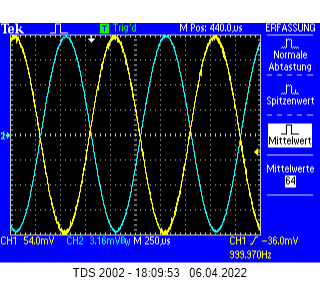
\includegraphics[width=\linewidth, height=10cm]{./figures/messungen/ohnekond24mv.png}
  %TODO caption
  \caption{Ohne Überbrückungskondensator}
  \label{fig:oszi_ohne_normal}
\end{figure}

\paragraph{Schaltung mit Überbrückungskondensator}
\begin{figure}[H]
  \centering
    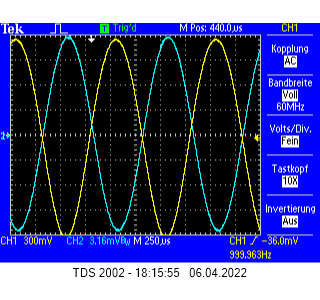
\includegraphics[width=\linewidth, height=10cm]{./figures/messungen/mitkond24mv.png}
  %TODO caption
  \caption{Mit Überbrückungskondensator}
  \label{fig:oszi_mit_normal}
\end{figure}


% 1.4 Überprüfen Sie die Übersteuerungsgrenze mit und ohne CE und nehmen Sie auch hier die
% Eingangspannung und die Ausgangsspannung im übersteuerten Betrieb mittels Oszilloskop auf.

\subsubsection{Übersteuerungsbetrieb}
%TODO Einfuegen von Bilder mit Messwerten
\paragraph{Schaltung ohne Überbrückungskondensator}
\begin{figure}[H]
  \centering
    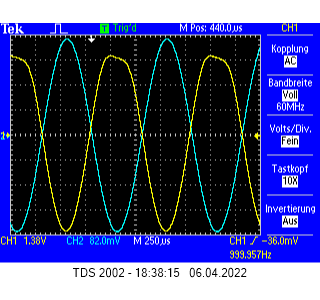
\includegraphics[width=\linewidth, height=10cm]{./figures/messungen/ohneuebergrenze.png}
  %TODO caption
  \caption{Ohne Überbrückungskondensator}
  \label{fig:oszi_ohne_uebersteuerung}
\end{figure}


\paragraph{Schaltung mit Überbrückungskondensator}

\begin{figure}[H]
  \centering
    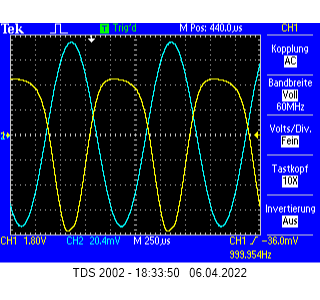
\includegraphics[width=\linewidth, height=10cm]{./figures/messungen/mituebergrenze.png}
  %TODO caption
  \caption{Mit Überbrückungskondensator}
  \label{fig:oszi_mit_uerbersteuerung}
\end{figure}

% 1.5 Variieren Sie nun die Frequenz und zeigen Sie die diesbezüglichen Grenzen der Schaltung.
% Diskutieren Sie mit Hilfe eines Oszilloskopbildes die Konsequenzen.
\subsubsection{Frequenzvariation}

Nun wurde die Frequenz des Eingangssignals varriert um die Untere- bzw.
Oberegrenzfrequenz zu finden und das Verhalten der Schaltung bei
Frequenzvariation zu untersuchen. Die Unteregrenzfrequenz somit bestimmt worden und in  
\autoref{fig:oszi_untergrenzfrequenz} ersichtlich.

%TODO Einfügen von Bilder mit Messwerten
\begin{figure}[H]
  \centering
    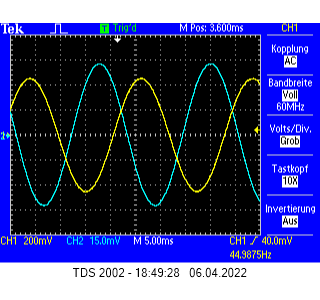
\includegraphics[width=\linewidth, height=10cm]{./figures/messungen/unteregrenze.png}
    \caption{Diese Abbildungen zeigt den zeitlichen Verlauf der Eingangs- (Blau) und
    Ausgangsspannung (Gelb) beim Betrieb an der unteren Grenzfrequenz (siehe Abbildung
  \SI{44.9875}{\hertz})}
  \label{fig:oszi_untergrenzfrequenz}
\end{figure}

% 1.6 Während Sie das Live-Oszilloskopbild betrachten, können Sie mittels Körpertemperatur das
% Metallgehäuse des Transistors erwärmen. Schauen Sie sich die Folgen genau an und diskutieren Sie
% diese.

% TODO konnte nicht gemacht werden

% 1.7 Bauen Sie die Schaltung ab, ordnen Sie die Bauteile wieder in die dafür vorgesehenen Boxen,
% schalten Sie alle Geräte die Sie verwendet haben aus und verlassen Sie den Platz so wie Sie
% ihn vorgefunden haben.

% TODO Besprechen. Hauen wir ein Bild von unserem sauberen Arbeitsplatz hinein?

% zu 4: Auswertung siehe EPM Skript nur Besprechung von Umformungen und 
% Sachen die man mit den Messungen machen muss damit man Conclusion und Wissen 
% gewinnen kann.
% Entsprechend der in Punkt 2. angegebenen Beziehungen (Formeln) ist aus
% den Messergebnissen in Punkt 5. das in Punkt 1. formulierte Endergebnis zu berechnen.
% Oft ist eine Ermittlung des Endergebnisses aus einer grafischen Darstellung bzw. eine grafi-
% sche Veranschaulichung zweckm ̈aßig. Dabei kann die Verwendung von Millimeterpapier oder
% Computerprogrammen hilfreich sein. Wenn eine Bearbeitung der Daten auf dem Computer
% erfolgt, sollte bei der Darstellung der Graphen eine sinnvolle Skalenteilung des Koordina-
% tensystems gemacht werden. Die Unsicherheitsbetrachtung f ̈ur die angegebenen Messwerte,
% sowie f ̈ur Zwischen- und Endergebnisse ist in diesem Abschnitt nachvollziehbar zu beschrei-
% ben. Dabei ist nach Kapitel 1 vorzugehen und insbesondere auf die Klassifizierung der
% Unsicherheit (Typ-A/B) und die Unsicherheitsfortpflanzung einzugehen.
\section{Auswertung}\label{sec:Auswertung}

\subsection{Simulation}

% 1.1 Start Ausarbeitung
\subsubsection{Schaltung ohne Überbrückungskondensator}


% 1.2 Stellen Sie eine Eingangs-Sinusspannung von 1 kHz mit einer Amplitude innerhalb der
% Übersteuerungstoleranzen ein, erzeugen Sie ein Simulation Profil (Time Domain) und nehmen Sie
% jeweils die Eingangsspannung und die Ausgangsspannung in einem Plot über die Zeit auf. Lassen Sie
% sich auch die Spannungen und Ströme im Schaltbild anzeigen um den Arbeitspunkt diskutieren zu
% können. Berechnen Sie daraus die simulierte Verstärkung und diskutieren Sie die beiden Diagramme
% und ihren Zusammenhang.
\paragraph{Verstärkung}

Es wurde aus den Simulationdaten von \textit{LTSPICE}, siehe
\autoref{fig:verlaufohnekond}, die Spitzenspannungen für $U_e$ und $U_a$
bestimmt wodurch mit \autoref{eq:verst} die Verstärkung $V_{u}'$ berechnet wurde:

\begin{equation}
  V_{u}' = 19
  \label{eq:sim_verst_ohne}
\end{equation}

% TODO 3D plot und erklaerung wie dieser gemacht wurde

% 1.3 Testen Sie wie hoch die maximale Eingangspannung werden darf bis der Transistor in der Simulation
% übersteuert. Übersteuern Sie ihn anschließend und nehmen Sie wieder die Eingangspannung sowie
% die Ausgangsspannung nach der Zeit auf und diskutieren Sie anhand dieses Plots die auftretenden
% Verzerrungen.

% 1.4 Erstellen Sie einen DC Sweep in Abhängigkeit der Temperatur und zeigen Sie die Änderung des
% Kollektorpotentials. Diskutieren Sie die Konsequenzen einer Temperaturerhöhung.

% 1.5 Nehmen Sie die Ausgangsspannung über der Zeit für verschiedene Temperaturen in einem
% Diagramm dar und diskutieren Sie diesen Plot.

% 2.1 Start Ausarbeitung
\subsubsection{Schaltung mit Überbrückungskondensator}


% 2.2 Stellen Sie eine Eingangs-Sinusspannung von 1 kHz mit einer Amplitude innerhalb der
% Übersteuerungstoleranzen ein, erzeugen Sie ein Simulation Profil (Time Domain) und nehmen Sie
% jeweils die Eingangsspannung und die Ausgangsspannung in einem Plot über die Zeit auf. Lassen Sie
% sich auch die Spannungen und Ströme im Schaltbild anzeigen um den Arbeitspunkt diskutieren zu
% können. Berechnen Sie daraus die simulierte Verstärkung und diskutieren Sie die beiden Diagramme
% und ihren Zusammenhang.
\paragraph{Verstärkung}

Es wurde aus den Simulationdaten von \textit{LTSPICE}, siehe
\autoref{fig:sim_mit_normal_eingang} und \autoref{fig:sim_mit_normal_ausgang},
die Spitzenspannungen für $U_e$ und $U_a$ bestimmt wodurch mit
\autoref{eq:verst} die Verstärkung mit Überbrückungskondensator $V_{u,C_{E}}'$
berechnet wurde.

\begin{equation}
  V_{u,C_{E}}' = 125
  \label{eq:sim_verst_mit}
\end{equation}

% TODO 3D plot und erklaerung wie dieser gemacht wurde
% 2.3 Testen Sie wie hoch die maximale Eingangspannung werden darf bis der Transistor in der Simulation
% übersteuert. Übersteuern Sie ihn anschließend und nehmen Sie wieder die Eingangspannung sowie
% die Ausgangsspannung nach der Zeit auf und diskutieren Sie anhand dieses Plots die auftretenden
% Verzerrungen.

% 2.4 Erstellen Sie einen DC Sweep in Abhängigkeit der Temperatur und zeigen Sie die Änderung des
% Kollektorpotentials. Diskutieren Sie die Konsequenzen einer Temperaturerhöhung.

% 2.5 Nehmen Sie die Ausgangsspannung über der Zeit für verschiedene Temperaturen in einem
% Diagramm dar und diskutieren Sie diesen Plot.


% 3.1 Auch wenn die Schaltung prinzipiell nicht dafür ausgerichtet ist − bauen Sie RE und CE aus und
% untersuchen Sie die Verstärkung und die Temperaturabhängigkeit des Kollektorpotentials ohne
% jegliche Rückkopplung. (Beachten Sie, dass der Arbeitspunkt dabei unvorteilhaft verschoben wird.)
\subsubsection{Schaltung ohne Emitterwiderstand \& Überbückungskondensator}

Es wurde aus den Simulationdaten von \textit{LTSPICE}, siehe
\autoref{fig:verlaufohnekondundre} die Spitzenspannungen für $U_e$ und $U_a$
bestimmt wodurch mit \autoref{eq:verst} die Verstärkung ohne Emitterwiderstand
und ohne Überbrückungskondensator $V_{u,\neg R_{E}}'$ berechnet wurde.

\begin{equation}
  V_{u,\neg R_{E}}' = 931
  \label{eq:sim_verst_ohne_ohne_re}
\end{equation}

\subsubsection{Verstärkung} \label{sec:ausverst}
Um die Verstärkung zu bestimmen, wurde über die Amplituden des zeitlichen
Verlaufs der Ausgangs- und Eingangsspannungen gemittelt und deren Verhältnis
gemäß \autoref{eq:verst} berechnet. Somit ergeben sich die Werte der Tabelle
\autoref{tab:verst_sim_alle} für die Verstärkungen der drei Schaltungen aus dem Abschnitt
\nameref{sec:Versuchsim}. 


%TODO: insert table with amplifications (ohne kond, mit kond, ohne kondundre)
\begin{table}[H]
  %TODO caption
  \caption{Tabelle mit allen ermittelten Verstärkungen \\
  $V_{u} \dots'$ Verstärkung ohne Überbrückungskondensator \\
  $V_{u,C_{E}} \dots'$   Verstärkung mit Überbrückungskondensator \\
  $V_{u,\neg R_{E}} \dots'$ Verstärkung ohne Emitterwiderstand und ohne Überbrückungskondensator 
  }
  \label{tab:verst_sim_alle}
  \centering
  \begin{tabular}{l|l}
  %TODO data
  $V_{u}'$            & 19 \\
  $V_{u,C_{E}}'$      & 125 \\
  $V_{u,\neg R_{E}}'$ & 931
  \end{tabular}
\end{table}



% 1.1 Bauen Sie die Schaltung am Steckboard gemäß der berechneten Parameter ohne den Kondensator CE
% auf. Nähern Sie sich bei Ihren berechneten Widerstandswerten durch Serienschaltung der
% vorhandenen Fixwiderstände der Reihe E12 auf ein vernünftiges Maß an. Führen sie den
% Eingangsspannungsteiler mit einem Fixwiderstand und einem Potentiometer aus um den
% Arbeitspunkt anpassen zu können. Notieren Sie die tatsächlich verwendeten Widerstandswerte
% (messen Sie hierfür die Widerstände aus, diese weichen nämlich teilweise erheblich von ihrem
% nominellen Wert ab).
\subsection{Steckbrett}

% TODO Braucht keine Auswertung 1.1? 


% 1.2 (Überprüfen der Schaltung durch einen Betreuer bevor Inbetriebnahme!)
% Verwenden Sie das Netzgerät für eine konstante Versorgungsspannung messen Sie das
% Kollektorpotential VC,A, stellen Sie es wenn nötig mit Hilfe des Potentiometers auf den gewünschten
% Wert ein. Protokollieren Sie die angepassten Widerstandswerte und die folgenden Größen UCE, UBE,
% VC, VB, IC, IB um den Arbeitspunkt evaluieren zu können.
Da ein Großteil, der Arbeitspunkt definierenden Größen, direkt gemessen werden
konnte, wird hier nur noch die fehlenden Größen mit den Messwerten aus
\autoref{tab:messugenarbeitspunkt} errechnet. Es sind nur noch der Basisstrom
$I_B$ und der Kollektorstrom $I_C$ zu bestimmen. Durch Verwendung
\autoref{eq:ohm} kann $I_C$ durch den Spannungsabfall über den
Kollektorwiderstand bestimmt werden. Da $I_B$ nichts anderes ist als die
Differenz von dem Strom durch $R_1$ und dem Strom durch $R_2$ (siehe
\autoref{fig:schaltungohnekond}) kann $I_B$ äquivalent zu $I_C$ berechnet
werden. Für die Fehlerfortpflanzung ist das Gaußsches Fehlerfortpflanzunggesetz
verwendet worden.

%TODO Einfuegen von Tabelle mit errechneten Werten
\begin{table}[H]
  %TODO caption
  \caption{ Tabelle mit den fehlenden zuerechnenden Größen des Arbeitspunkts \\
  $I_C \dots$ Kollektorstrom \\
  $I_B \dots$ Basisstrom 
  }
  \label{tab:aus_arbeitspunkt_daten}
  \centering
  \begin{tabular}[c]{l|l}
  %TODO
    $I_C$ & \SI{4.29(12)}{\milli\ampere} \\
    $I_B$ & \SI{6(4)}{\micro\ampere} \\
  \end{tabular}
\end{table}


% 1.3 (Überprüfen der Schaltung durch einen Betreuer bevor Inbetriebnahme!)
% Stellen Sie nun eine sinusförmige Wechselspannung mit Hilfe des Funktionsgenerators von 1kHz
% ein und benützen Sie dieses Signal als Eingangssignal für Ihre Schaltung. Stellen Sie nun die
% Eingangspannung und die Ausgangsspannung mittels Oszilloskop dar und zwar jeweils mit und
% ohne CE. Laden Sie die Bilder oder wahlweise die Daten mittels dem Programm Open Choice
% Desktop herunter, diskutieren Sie diese, berechnen Sie die Verstärkungen und vergleichen Sie die
% Daten mit der Simulation.
\subsubsection{Normalbetrieb}
%TODO Errechnen von der Verstaerkung 
Die Verstärkungsfaktoren wurden analog wie für die Simulation im
vorigen Abschnitt \nameref{sec:ausverst} ermittelt. Diese ergeben sich zu

\paragraph{Schaltung ohne Überbrückungskondensator}

Da bei der Aufnahme der Daten das Oszilloskop so eingestellt wurde, dass das
Signal die "Full-Scale" komplett ausnutz, kann die Verstärkung $V_{u}'$ durch
Division der Volts per Division vom Eingangs- und Ausgangsssignals, welche im
Oszillogramm, siehe \autoref{fig:oszi_ohne_normal}, ersichtlich sind, errechnet
werden.

\begin{equation}
  V_{u}' = 17
  \label{eq:oszi_verst_ohne}
\end{equation}

\paragraph{Schaltung mit Überbrückungskondensator}

Da bei der Aufnahme der Daten das Oszilloskop so eingestellt wurde, dass das
Signal die "Full-Scale" komplett ausnutz, kann die Verstärkung $V_{u,C_{E}}'$
durch Division der Volts per Division vom Eingangs- und Ausgangsssignals,
welche im Oszillogramm, siehe \autoref{fig:oszi_mit_normal}, ersichtlich sind,
errechnet werden.

\begin{equation}
  V_{u,C_{E}}' = 95
  \label{eq:oszi_verst_mit}
\end{equation}

% 1.4 Überprüfen Sie die Übersteuerungsgrenze mit und ohne CE und nehmen Sie auch hier die
% Eingangspannung und die Ausgangsspannung im übersteuerten Betrieb mittels Oszilloskop auf.
\subsubsection{Übersteuerungsbetrieb}
%TODO Errechnen von der Verstaerkung?????
\paragraph{Schaltung ohne Überbrückungskondensator}

\paragraph{Schaltung mit Überbrückungskondensator}

% 1.5 Variieren Sie nun die Frequenz und zeigen Sie die diesbezüglichen Grenzen der Schaltung.
% Diskutieren Sie mit Hilfe eines Oszilloskopbildes die Konsequenzen.
\subsubsection{Frequenzvariation}
% TODO Braucht keine Auswertung? 

% 1.6 Während Sie das Live-Oszilloskopbild betrachten, können Sie mittels Körpertemperatur das
% Metallgehäuse des Transistors erwärmen. Schauen Sie sich die Folgen genau an und diskutieren Sie
% diese.

% TODO konnte nicht gemacht werden

% 1.7 Bauen Sie die Schaltung ab, ordnen Sie die Bauteile wieder in die dafür vorgesehenen Boxen,
% schalten Sie alle Geräte die Sie verwendet haben aus und verlassen Sie den Platz so wie Sie
% ihn vorgefunden haben.

% TODO Besprechen. Hauen wir ein Bild von unserem sauberen Arbeitsplatz hinein?



% zu 5: Diskussion und Zusammenfassung
% In der Zusammenfassung stehen noch einmal die wichtigsten Messergebnisse, wobei auf Tabellen und
% Abbildungen nur verwiesen werden soll. Die Ergebnisse sind auch zu diskutieren. Insbesondere müssen
% Abweichungen zwischen Simulation und praktischer Durchführung diskutiert werden.
\section{Diskussion und Zusammenfassung}\label{sec:Diskussion} 


% 1.2 Stellen Sie eine Eingangs-Sinusspannung von 1 kHz mit einer Amplitude innerhalb der
% Übersteuerungstoleranzen ein, erzeugen Sie ein Simulation Profil (Time Domain) und nehmen Sie
% jeweils die Eingangsspannung und die Ausgangsspannung in einem Plot über die Zeit auf. Lassen Sie
% sich auch die Spannungen und Ströme im Schaltbild anzeigen um den Arbeitspunkt diskutieren zu
% können. Berechnen Sie daraus die simulierte Verstärkung und diskutieren Sie die beiden Diagramme
% und ihren Zusammenhang.

% 1.3 Testen Sie wie hoch die maximale Eingangspannung werden darf bis der Transistor in der Simulation
% übersteuert. Übersteuern Sie ihn anschließend und nehmen Sie wieder die Eingangspannung sowie
% die Ausgangsspannung nach der Zeit auf und diskutieren Sie anhand dieses Plots die auftretenden
% Verzerrungen.

% 1.4 Erstellen Sie einen DC Sweep in Abhängigkeit der Temperatur und zeigen Sie die Änderung des
% Kollektorpotentials. Diskutieren Sie die Konsequenzen einer Temperaturerhöhung.

% 1.5 Nehmen Sie die Ausgangsspannung über der Zeit für verschiedene Temperaturen in einem
% Diagramm dar und diskutieren Sie diesen Plot.

% 2.2 Stellen Sie eine Eingangs-Sinusspannung von 1 kHz mit einer Amplitude innerhalb der
% Übersteuerungstoleranzen ein, erzeugen Sie ein Simulation Profil (Time Domain) und nehmen Sie
% jeweils die Eingangsspannung und die Ausgangsspannung in einem Plot über die Zeit auf. Lassen Sie
% sich auch die Spannungen und Ströme im Schaltbild anzeigen um den Arbeitspunkt diskutieren zu
% können. Berechnen Sie daraus die simulierte Verstärkung und diskutieren Sie die beiden Diagramme
% und ihren Zusammenhang.

% 2.3 Testen Sie wie hoch die maximale Eingangspannung werden darf bis der Transistor in der Simulation
% übersteuert. Übersteuern Sie ihn anschließend und nehmen Sie wieder die Eingangspannung sowie
% die Ausgangsspannung nach der Zeit auf und diskutieren Sie anhand dieses Plots die auftretenden
% Verzerrungen.

% 2.4 Erstellen Sie einen DC Sweep in Abhängigkeit der Temperatur und zeigen Sie die Änderung des
% Kollektorpotentials. Diskutieren Sie die Konsequenzen einer Temperaturerhöhung.

% 2.5 Nehmen Sie die Ausgangsspannung über der Zeit für verschiedene Temperaturen in einem
% Diagramm dar und diskutieren Sie diesen Plot.

% 3.1 Auch wenn die Schaltung prinzipiell nicht dafür ausgerichtet ist − bauen Sie RE und CE aus und
% untersuchen Sie die Verstärkung und die Temperaturabhängigkeit des Kollektorpotentials ohne
% jegliche Rückkopplung. (Beachten Sie, dass der Arbeitspunkt dabei unvorteilhaft verschoben wird.)
% ERLANGTE ERKENNTNIS!

% 1.3 (Überprüfen der Schaltung durch einen Betreuer bevor Inbetriebnahme!)
% Stellen Sie nun eine sinusförmige Wechselspannung mit Hilfe des Funktionsgenerators von 1kHz
% ein und benützen Sie dieses Signal als Eingangssignal für Ihre Schaltung. Stellen Sie nun die
% Eingangspannung und die Ausgangsspannung mittels Oszilloskop dar und zwar jeweils mit und
% ohne CE. Laden Sie die Bilder oder wahlweise die Daten mittels dem Programm Open Choice
% Desktop herunter, diskutieren Sie diese, berechnen Sie die Verstärkungen und vergleichen Sie die
% Daten mit der Simulation.
Man achte hierbei auf die Volts per division bei Gleicher Eingangsspannung
erzeugt die Schaltung mit Kondensator eine um fast 6-fache größere Verstärkung.

Die für die Simulation bestimmten Verstärkungen der Schaltungen sind der
Tabelle \autoref{tab:verst_sim_alle} zu entnehmen. Die reale Verstärkung der Schaltung
am Steckbrett ergibt sich zu xxx.

\newpage

\printbibliography

\listoffigures

\listoftables



\end{document}

